% \documentclass[journal, 12pt, onecolumn, draftclsnofoot]{IEEEtran} %journal draft
\documentclass[conference]{IEEEtran} %conference draft

\usepackage[linesnumbered,vlined,ruled]{algorithm2e}
\usepackage{algorithmic}
\usepackage{etoolbox}
\ifCLASSOPTIONcompsoc
  % IEEE Computer Society needs non-compress option
  % requires cite.sty v4.0 or later (November 2003)
  \usepackage[nocompress]{cite}
\else
  % normal IEEE
  \usepackage{cite}
\fi
\usepackage{graphicx}
\graphicspath{ {./images/} }
\usepackage{amsmath,amsthm,amssymb,amsfonts}
\usepackage{mathtools}
\usepackage[dvipsnames]{xcolor}
\usepackage{dcolumn}
\usepackage[utf8]{inputenc}
\usepackage{soul}
\usepackage{array}
\usepackage{tabulary}
\usepackage{bbm}
\DeclareMathAlphabet{\mathpzc}{OT1}{pzc}{m}{it}
%---------------------------------------------------------------%
%% the pretty \widebar symbol: 
\makeatletter
\let\save@mathaccent\mathaccent
\newcommand*\if@single[3]{%
  \setbox0\hbox{${\mathaccent"0362{#1}}^H$}%
  \setbox2\hbox{${\mathaccent"0362{\kern0pt#1}}^H$}%
  \ifdim\ht0=\ht2 #3\else #2\fi
  }
%The bar will be moved to the right by a half of \macc@kerna, which is computed by amsmath:
\newcommand*\rel@kern[1]{\kern#1\dimexpr\macc@kerna}
%If there's a superscript following the bar, then no negative kern may follow the bar;
%an additional {} makes sure that the superscript is high enough in this case:
\newcommand*\widebar[1]{\@ifnextchar^{{\wide@bar{#1}{0}}}{\wide@bar{#1}{1}}}
%Use a separate algorithm for single symbols:
\newcommand*\wide@bar[2]{\if@single{#1}{\wide@bar@{#1}{#2}{1}}{\wide@bar@{#1}{#2}{2}}}
\newcommand*\wide@bar@[3]{%
  \begingroup
  \def\mathaccent##1##2{%
%Enable nesting of accents:
    \let\mathaccent\save@mathaccent
%If there's more than a single symbol, use the first character instead (see below):
    \if#32 \let\macc@nucleus\first@char \fi
%Determine the italic correction:
    \setbox\z@\hbox{$\macc@style{\macc@nucleus}_{}$}%
    \setbox\tw@\hbox{$\macc@style{\macc@nucleus}{}_{}$}%
    \dimen@\wd\tw@
    \advance\dimen@-\wd\z@
%Now \dimen@ is the italic correction of the symbol.
    \divide\dimen@ 3
    \@tempdima\wd\tw@
    \advance\@tempdima-\scriptspace
%Now \@tempdima is the width of the symbol.
    \divide\@tempdima 10
    \advance\dimen@-\@tempdima
%Now \dimen@ = (italic correction / 3) - (Breite / 10)
    \ifdim\dimen@>\z@ \dimen@0pt\fi
%The bar will be shortened in the case \dimen@<0 !
    \rel@kern{0.6}\kern-\dimen@
    \if#31
      \overline{\rel@kern{-0.6}\kern\dimen@\macc@nucleus\rel@kern{0.4}\kern\dimen@}%
      \advance\dimen@0.4\dimexpr\macc@kerna
%Place the combined final kern (-\dimen@) if it is >0 or if a superscript follows:
      \let\final@kern#2%
      \ifdim\dimen@<\z@ \let\final@kern1\fi
      \if\final@kern1 \kern-\dimen@\fi
    \else
      \overline{\rel@kern{-0.6}\kern\dimen@#1}%
    \fi
  }%
  \macc@depth\@ne
  \let\math@bgroup\@empty \let\math@egroup\macc@set@skewchar
  \mathsurround\z@ \frozen@everymath{\mathgroup\macc@group\relax}%
  \macc@set@skewchar\relax
  \let\mathaccentV\macc@nested@a
%The following initialises \macc@kerna and calls \mathaccent:
  \if#31
    \macc@nested@a\relax111{#1}%
  \else
%If the argument consists of more than one symbol, and if the first token is
%a letter, use that letter for the computations:
    \def\gobble@till@marker##1\endmarker{}%
    \futurelet\first@char\gobble@till@marker#1\endmarker
    \ifcat\noexpand\first@char A\else
      \def\first@char{}%
    \fi
    \macc@nested@a\relax111{\first@char}%
  \fi
  \endgroup
}
\makeatother
%---------------------------------------------------------------%
\newtheorem{definition}{Definition}   % 
\theoremstyle{definition}             % alter theorem style: <definition>
\newtheorem{program}{Program}         % [program]
\newtheorem{assumption}{Assumption}   % [assumption]
\newtheorem{example}{Example}         % [example]
\newtheorem{Algorithm}{Algorithm}     % [algorithm]
\newtheorem{policy}{Policy}           % [policy]
\newtheorem{problem}{Problem}         % [problem]
\theoremstyle{remark}                 % alter theorem style: <remark>
\newtheorem{remark}{Remark}           % [remark]
\theoremstyle{plain}                  % alter theorem style: <plain>
\newtheorem{theorem}{Theorem}         % [theorem]
\newtheorem{lemma}{Lemma}             % [lemma]
\newtheorem{corollary}{Corollary}     % [corollary]
%---------------------------------------------------------------%
\newcommand{\slide}[1]{{\mathbf{#1}}} %\overset{\rightarrow}
\newcommand{\eq}{=}
\newcommand{\domR}{\mathbb{R}}
\newcommand{\domZ}{\mathbb{Z}_{*}}
\newcommand{\domP}{\mathbb{Z}_{*}}
\newcommand{\vecOne}{\mathbf{1}}
\newcommand{\indicator}{\mathbbm{1}}
\newcommand{\mat}{\mathbf}
\newcommand{\Poisson}{\text{Poisson}}
\newcommand{\Bernoulli}{\text{Bernoulli}}
\newcommand{\define}{\triangleq}
\newcommand{\leadto}{\Rightarrow}
\newcommand{\vecG}{\boldsymbol}
\renewcommand{\vec}{\mathbf}
\newcommand{\Baseline}{\mathbf{\Pi}}
\newcommand{\T}{{T_{\max}}}
\newcommand{\C}{\mathcal{C}}
\renewcommand{\d}{\mathpzc{d}}
\renewcommand{\u}{\mathpzc{u}}
\renewcommand{\L}{\mathcal{L}}
\DeclarePairedDelimiter\ceil{\lceil}{\rceil}
\DeclarePairedDelimiter\floor{\lfloor}{\rfloor}
\DeclarePairedDelimiter{\set}{\{}{\}}
\DeclarePairedDelimiter{\norm}{|}{|}
\DeclarePairedDelimiter{\Inorm}{\|}{\|_1}
\DeclarePairedDelimiter{\paren}{(}{)}
\DeclarePairedDelimiter{\Paren}{\bigg(}{\bigg)}
\DeclarePairedDelimiter{\bracket}{[}{]}
\DeclarePairedDelimiter{\Bracket}{\bigg[}{\bigg]}
\DeclarePairedDelimiter{\Brace}{\bigg\{}{\bigg\}}
%----------------------------------------------------------%
%% mathematical symbols
\newcommand{\tjSet}{\mathcal{W}}
\newcommand{\carSet}{\mathcal{M}}
\newcommand{\Stat}{\mathbf{S}}
\newcommand{\Policy}{\vecG{\Omega}}
\newcommand{\TransD}{\mathbf{D}}
\newcommand{\Diag}{\text{Diag}}
%----------------------------------------------------------%
%% terminology symbols
\newcommand{\IAV}{DCV}
\newcommand{\IAVs}{\IAV{s}}
\newcommand{\IAVFullname}{data collection vehicle}
\newcommand{\IAVFullnames}{\IAVFullname{s}}
\newcommand{\fwName}{FedCars}
%----------------------------------------------------------%
%% extended comments
\newcommand{\fixit}[1]{{\leavevmode\color{red}#1}}
\newcommand{\nice}[1]{{\leavevmode\color{black}#1}}
\newcommand{\accept}[1]{#1}
\newcommand{\delete}[2]{}
\newcommand{\needref}[1]{{\leavevmode\color{red}[#1]}}
%---------------------------------------------------------------%
%% review comments
\newcommand{\extension}[1]{} %{{ \leavevmode\color{blue}#1 }}
\newcommand{\transition}[1]{{ \leavevmode\color{black}#1 }}
\newcommand{\wangr}[1]{{\leavevmode\color{orange}#1}}
\newcommand{\hongyc}[1]{{\leavevmode\color{purple}#1}}
\newcommand{\tann}[1]{{\leavevmode\color{blue}#1}}
%---------------------------------------------------------------%

%---------------------------------------------------------------%
\def\BibTeX{{\rm B\kern-.05em{\sc i\kern-.025em b}\kern-.08em
    T\kern-.1667em\lower.7ex\hbox{E}\kern-.125emX}}
%---------------------------------------------------------------%
\IEEEoverridecommandlockouts
\begin{document}
    \title{
      {\fwName}: An Efficient Scheduling Framework for In-Vehicle Federated Learning 
      Integrated with CARLA-Cosimulation
    }
    \author{
        Yuncong~Hong,
        Bojie~Lv,
        Shuai~Wang,
        Rui~Wang,
        Haisheng~Tan,
        Francis~C.M.~Lau
        \thanks{
          Y. Hong is with Southern University of Science and Technology (SUSTech), and the University of Hong Kong (HKU) (email: ychong@cs.hku.hk).
        }
        \thanks{
          B. Lv and R. Wang are with the Department of Electrical and Electronic Engineering, Southern University of Science and Technology (SUSTech), Shenzhen, China (email: lvbj@mail.sustech.edu.cn, wang.r@sustech.edu.cn).
        }
        \thanks{
          S. Wang is with the Shenzhen Institute of Advanced Technology, Chinese Academy of Sciences (CAS), Shenzhen 518055, China (email: s.wang@siat.ac.cn).
        }
        \thanks{
          H. Tan is with the LINKE Lab,  University of Science and Technology of China (USTC), Hefei, China (email: hstan@ustc.edu.cn).
        }%
        \thanks{
          F.C.M. Lau is with the Department of Computing Science, the University of Hong Kong (HKU), Hong Kong (email: fcmlau@cs.hku.hk).
        }%
    }

    % \begin{abstract}
    % the background
    % CARLA is a well-established open-source simulator for high-fidelity emulation of self-driving systems, which has been widely used for the development and validation of machine learning models on autonomous driving.
    %<*tag:abstract>
    \revise{
        Federated learning on vehicles has been widely considered in autonomous driving. The model uploading of federated learning is time-consuming, which motivates the transmission optimization that exploits the mobility of vehicles.
    }%
    In this paper, an optimization framework integrated with the high-fidelity traffic simulator CARLA, namely {\fwName}, is proposed for the scheduling of model uploading in a Vehicle-to-Infrastructure (V2I) network.
    Specifically, a group of {\IAVFullnames} ({\IAVs}) move along their planned routes with random velocities to collect sensor data and train a model via federated learning, where the uplink model transmission of multiple {\IAVs} in one learning iteration is jointly optimized.
    % the platform
    We first develop the {\fwName} simulator from CARLA, to obtain a high-fidelity trajectory dataset of {\IAVs} in the considered traffic scenario, and train the transition probabilities of the {\IAVs}' locations.
    % the problem
    Hence, the uplink transmission time and power of all {\IAVs} in all the time slots can be formulated as a finite-horizon Markov Decision Process (MDP), where the prediction of {\IAVs}' future locations is exploited to minimize a weighted sum of the average model uploading time and the average energy consumption.
    \revise{
        A low-complexity {\fwName} optimizer with a non-trivial performance bound is then proposed, where the optimization consists of global transmission time allocation and local power allocation. The former periodically allocates the transmission time for the remaining time slots according to an average trajectory. Hence, the power allocation of all {\IAVs} can be decoupled to local finite-horizon MDPs in the latter. They can be solved by one-step policy improvement with low computational complexity.
    }%
    The simulation results show that the proposed solution framework can achieve both a significant performance gain over the baselines and a flexible trade-off between performance and complexity.
    %</tag:abstract>
\end{abstract}

\begin{IEEEkeywords}
    Federated edge learning (FEEL),
    CARLA,
    Approximate MDP.
\end{IEEEkeywords}

    \maketitle
    \begin{abstract}
    % the background
    % CARLA is a well-established open-source simulator for high-fidelity emulation of self-driving systems, which has been widely used for the development and validation of machine learning models on autonomous driving.
    %<*tag:abstract>
    \revise{
        Federated learning on vehicles has been widely considered in autonomous driving. The model uploading of federated learning is time-consuming, which motivates the transmission optimization that exploits the mobility of vehicles.
    }%
    In this paper, an optimization framework integrated with the high-fidelity traffic simulator CARLA, namely {\fwName}, is proposed for the scheduling of model uploading in a Vehicle-to-Infrastructure (V2I) network.
    Specifically, a group of {\IAVFullnames} ({\IAVs}) move along their planned routes with random velocities to collect sensor data and train a model via federated learning, where the uplink model transmission of multiple {\IAVs} in one learning iteration is jointly optimized.
    % the platform
    We first develop the {\fwName} simulator from CARLA, to obtain a high-fidelity trajectory dataset of {\IAVs} in the considered traffic scenario, and train the transition probabilities of the {\IAVs}' locations.
    % the problem
    Hence, the uplink transmission time and power of all {\IAVs} in all the time slots can be formulated as a finite-horizon Markov Decision Process (MDP), where the prediction of {\IAVs}' future locations is exploited to minimize a weighted sum of the average model uploading time and the average energy consumption.
    \revise{
        A low-complexity {\fwName} optimizer with a non-trivial performance bound is then proposed, where the optimization consists of global transmission time allocation and local power allocation. The former periodically allocates the transmission time for the remaining time slots according to an average trajectory. Hence, the power allocation of all {\IAVs} can be decoupled to local finite-horizon MDPs in the latter. They can be solved by one-step policy improvement with low computational complexity.
    }%
    The simulation results show that the proposed solution framework can achieve both a significant performance gain over the baselines and a flexible trade-off between performance and complexity.
    %</tag:abstract>
\end{abstract}

\begin{IEEEkeywords}
    Federated edge learning (FEEL),
    CARLA,
    Approximate MDP.
\end{IEEEkeywords}


    \section{Introduction}
\label{sec:introduction}
%NOTE: (1) federated learning for autonomous driving
Deep learning for autonomous driving \cite{ad-survey} has raised significant communication and computation burdens to wireless edge computing systems. This is because the raw data for model training collected on {\IAVFullnames} ({\IAVs}) is up to terabytes.
\revise{
    Fortunately, vehicular federated learning \cite{icra21-invs} could suppress unnecessary cost of data communication by uploading the locally trained models \cite{vfl-survey,feel-wangs,comst22-balkus,tiv23-chellapandi}.
}%
Nevertheless, model uploading in federated learning still consumes significant transmission time and energy.
In this paper, we would like to investigate the efficient model uploading techniques in a Vehicle-to-Infrastructure (V2I) network by exploiting the prediction on {\IAVs}' random trajectories.

\subsection{Related Works}
%NOTE: (2) related works for FL on vehicles
\revise{
    The federated learning on vehicles has been widely studied in the literature, where the communication scheduling is essential \cite{feel-wangs, comst22-balkus, tiv23-chellapandi}.
    Unlike the works that considered the communication scheduling for the federated learning in quasi-static scenarios \cite{Access19-Xu, iotj22-he, jsac23-du, tmc24-shen, tmc24-xu}, the communication and computation scheduling for vehicular networks is tightly coupled with the vehicles' trajectories.
    For example, the works \cite{tvt21-yang, tmc21-saputra, tits22-liu, tvt22-lee} studied the client selection strategy of the vehicles to alleviate the communication burden and thus improve the training efficiency, but did not optimize the transmission scheduling.

    % deterministic optimization for data uploading or offloading
    There have been a number of works that consider the joint optimization of communication and edge learning (or edge computing) in vehicle networks with deterministic trajectories \cite{Globecom18-Wang, TITS21-Xiao, IOTJ22-Lv, JSAC23-Pervej, TVT22-Hui, ICC23-Bansal, tvt21-zhao, tvt22-shinde, tits22-taik, jsac23-zhang,tmc23-zhang}.
    For example, in \cite{Globecom18-Wang}, the scenario of multiple vehicles moving along a unidirectional road at a constant speed and offloading the computation tasks to a base station (BS) was considered, where a heuristic scheme was proposed to suppress the delay of task offloading via Vehicle-to-Vehicle (V2V) communication.
    In \cite{TITS21-Xiao}, the weighted sum of time and energy consumption in vehicular federated learning was minimized, where the velocities of vehicles and the transmission data rate were assumed to be constant.
    Both \cite{jsac23-zhang} and \cite{tmc23-zhang} considered time-varying velocities of vehicles, where the former focused on the downlink broadcasting for the vehicular platoon, and the latter jointly optimized the transmission power and local model accuracy in the worst case.
}%

% stochastic optimization for offloading
In fact, the actual velocities of the vehicles are random, depending on the road map, population distribution, working hours, car-holding rate, driving habits and etc. The above scheduling design based on deterministic optimization could not be directly applied, as scheduling with random trajectory is usually a stochastic optimization problem.
There have been limited works on the scheduling of data communication or edge computing in vehicle networks with random trajectory
\cite{TVT18-Ni, Access19-Liu, TVT19-Liu, WC16-Salahuddin, TITS16-Wang, FGCS23-Sethi}.
For example in \cite{TVT18-Ni}, a hybrid Vehicle-to-Vehicle (V2V) and Vehicle-to-Infrastructure (V2I) network was considered with random inter-vehicle distance, where a heuristic strategy was proposed to cluster the vehicles and maximize the expected communication capacity.
In \cite{Access19-Liu}, continuous task offloading from single vehicle to multiple edge servers was optimized via the Q-learning where the average task turn around time was considered as the minimization objective. However, it is difficult to extend the Q-learning method to multi-vehicle scenario, due to the curse of dimensionality.
In \cite{TVT19-Liu}, the scenario that both fixed and vehicular servers would provide computation service to multiple user equipment was investigated. The Deep Q-Network (DQN) was leveraged to train the offloading and power allocation decisions, such that the average total communication and computation cost of all UEs was minimized. However, the model training might be of significant computational complexity, and the performance can hardly be bounded analytically with the method of DQN. Moreover, the models of random traffic in the above works might be too ideal to fit the real-world applications.
Therefore, there are still some open issues in the scheduling algorithm design for vehicle networks:
\begin{enumerate}
    \item How to depict the randomness of vehicular trajectory resembling the real-world statistics, instead of assuming it in a trivial form like Gaussian distribution?
    \item How to efficiently and reliably handle long-term and large-scale online resource allocation for vehicle networks with random traffic?
\end{enumerate}

\subsection{Our Contributions}

%<*tag:contribution>
To shed some light on the above issues, we particularly consider the scenario of in-vehicle federated learning, and propose an optimization framework with a high-fidelity traffic simulator, namely {\fwName}, for scheduling of the model uploading. 
\revise{
    Specifically, the uplink transmission time and power of multiple vehicles in a sequence of time slots are jointly scheduled to complete their model uploading.
}%
Due to the random trajectories of the vehicles, the scheduling design is a finite-horizon Markov Decision Process (MDP), where the complexity of the optimal solution grows exponentially with respect to the vehicle number \cite{mdp-cui,mdp-zhou}. The {\fwName} aims to exploit the statistical knowledge on the trajectories of vehicles and provide a low-complexity scheduling solution with good performance, where the contributions are summarized below.
\begin{itemize}
    \item We develop the {\fwName} simulator to obtain high-fidelity trajectory datasets of {\IAVs} in customizable traffic scenarios, so that the random trajectories of vehicles can be modeled as Markov chains via statistical learning and predicted in online scheduling.
    \revise{
    \item We propose a novel two-time scale solution algorithm, namely {\fwName} optimizer, to search for a suboptimal policy with low complexity. Note that the uplink scheduling of multiple vehicles is coupled due to the transmission time allocation. In the proposed solution, the complicated time allocation for the remaining model uploading is updated in a large time scale (every $N$ time slots). Given the time allocation, the power allocation of a DCV in each time slot (small time scale) can be calculated locally.
    \item A non-trivial performance bound is derived for the above two-time scale solution algorithm. The simulation results show that the {\fwName} optimizer outperforms various baselines, and achieves good balance between computational complexity and performance.
    }
\end{itemize}
%</tag:contribution>
The remainder of this paper is organized as follows.
In Section \ref{sec:model}, the traffic model of {\IAVs}, as well as the models of uplink queuing and data transmission, is described.
In Section \ref{sec:formulation}, the communication scheduling problem is formulated as a finite-horizon MDP, where the structure and challenge of optimal solution is discussed.
In Section \ref{sec:framework}, the {\fwName} simulator and the statistical learning for the vehicles' random trajectories are elaborated.
Then, the {\fwName} optimizer is introduced in Section \ref{sec:new_framework}, \ref{sec:kernel-policy} and \ref{sec:local-policy}.
Finally, the numerical simulation is presented in Section \ref{sec:simulation} and the conclusion is drawn in Section \ref{sec:conclusion}.

In this paper, we use the following notations:
non-bold letters (e.g., $a, A$) are used to denote scalar values,
bold lowercase letters (e.g., $\vec{a}$) are used to denote column vectors,
bold uppercase letters (e.g., $\mat{A}$) are used to denote matrices,
and calligraphic letters (e.g., $\mathcal{A}$) are used to denote sets.
$(\mat{A})_{i,j}$ denotes the $(i,j)$-th entry of the matrix $\mat{A}$.
$[a_{j}]_{j}$ with $j\in \mathcal{J}$ denotes the column vector whose entries' indexes take values from sets $\mathcal{J}$ in ascending order; $[a_{i,j}]_{i,j}$ with $i\in \mathcal{I}$ and  $j\in \mathcal{J}$ denotes the matrix.
$\|{\vec{a}}\|_2$ denote the L2-norm of vector $\vec{a}$.
$\indicator[\cdot]$ is the indicator function which is equal to $1$ when the inner statement is true and $0$ otherwise.

    % \input{src/02b-motivation}
    \section{System Model}
\label{sec:model}

\begin{figure}[htp!]
    \centering
    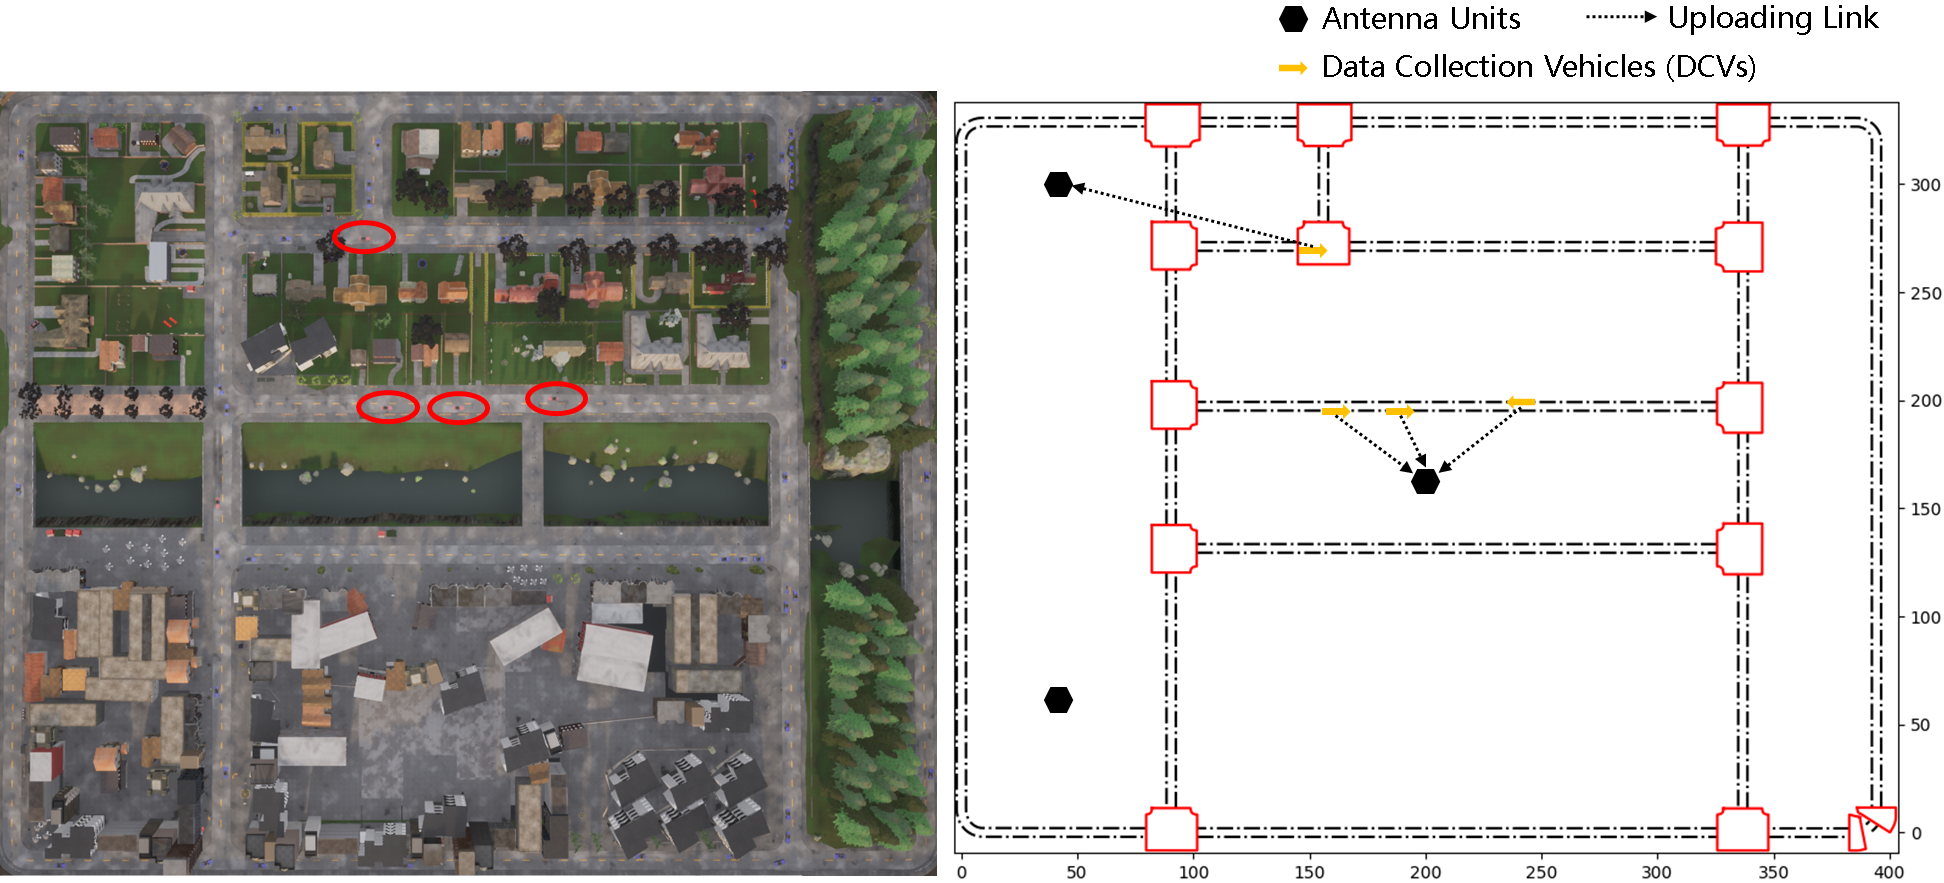
\includegraphics[width=0.45\textwidth]{fig-traffic-demo.png}
    \caption{Illustration of a road map example generated by CARLA.}
    \label{fig:town_map}
\end{figure}

In this paper, the scheduling of model uploading in a vehicular federated learning system is considered, which consists of $M$ {\IAVs} deployed with multi-modal sensors.
Denote the set of {\IAVs} as $\carSet = \set{1, \dots, M}$.
Each {\IAV} collects the sensing data for the cooperative training of a deep neural network, e.g., SECOND \cite{SECOND}, in a federated learning manner \cite{FedAvg}.
This is one of the typical machine learning scenario in the application of autonomous driving as elaborated in \cite{icra21-invs}.
In each training iteration, all the {\IAVs} first train their local models and then upload the trained models to an edge server for model aggregation via cellular uplink.
The aggregated model is then broadcast to the {\IAVs} for local training of next iteration until the convergence.
We particularly consider the uplink transmission scheduling in one iteration, where the {\IAVs}' mobility is exploited to save the transmission energy and suppress the model uploading time.

As an example illustrated in Fig.\ref{fig:town_map}, $M$ {\IAVs} are distributed at different positions of a road network.
They are moving along predetermined routes respectively, but their velocities are time-varying and random.
The route of the $m$-th {\IAV} ($\forall m\in\carSet$) is quantized into a sequence of waypoints denoted as
\begin{align*}
    \tjSet_{m} \define \Paren{ \vec{w}_{m,1}, \dots, \vec{w}_{m,|\tjSet_{m}|} },
\end{align*}
where $\vec{w}_{m,i} \in \domR^2$ denotes the coordinates of the $i$-th waypoint,
$|\tjSet_m|$ denotes the cardinality of $\tjSet_m$.

The system time is organized by time slots, each with a duration of $T_s$ seconds.
In the $t$-th time slot, the location of the $m$-th {\IAV} is denoted as $\vec{d}_{m,t} \in \tjSet_{m}$, and the trajectory of the $m$-th {\IAV} is represented by its locations in all the time slots, denoted by the stochastic process
\begin{align*}
    \vec{L}_{m} \define \Paren{ \vec{d}_{m,1}, \vec{d}_{m,2}, \dots }.
\end{align*}
%<*tag:route>
\revise{
    Note that although both the route and the trajectory consist of a sequence of waypoints, they are different. The sequence of waypoints for a route, say $\tjSet_{m}$, represents a path from location $\vec{w}_{m,1}$ to location $\vec{w}_{m,|\tjSet_{m}|}$. There is no velocity information for a route. 
    On the other hand, the sequence of waypoints for a trajectory represents the locations of a {\IAV} in different time slots. For example, a {\IAV} may stay at the same waypoint in two adjacent time slots due to heavy traffic.
    Thus, the velocity information can be deduced from the trajectory.
    Due to the random nature of traffic, the trajectory of a {\IAV} moving along a route is non-deterministic.
}%
%</tag:route>

In this paper, we approximate the trajectories of all {\IAVs} $\set{ \vec{L}_{m} | \forall m\in\carSet }$ as time-invariant Markov chains with the transition matrices
$\set{ \TransD_{m} \in \domR^{|\tjSet_{m}| \times |\tjSet_{m}|} | \forall m\in\carSet }$, where $\vec{D}_{m}$ represents the transition matrix of the $m$-th {\IAV}.
The entries of the transition matrix $\TransD_{m}$ are defined as follows:
\footnote{
    A sufficient number of waypoints is selected for each route, such that the last waypoint is never reached at the end of the model uploading.
    For example, the uploading of the $m$-th {\IAV} always completes before arriving at the waypoint $\vec{w}_{m,|\tjSet_m|}$.
}
\begin{align}
     \Paren{\TransD_{m}}_{i,j} \define \Pr\Bracket{ \vec{w}_{m,j} | \vec{w}_{m,i} }, \forall i,j.
    \label{eqn:trans_mat}
\end{align}

Without loss of generality, the local model training and uploading of the considered iteration starts from the $1$-st time slot.
Due to the heterogeneous computation capabilities of the {\IAVs}, the local training time of the {\IAVs} may be different.
It is assumed that the local training time of the $m$-th {\IAV} is $T_{\text{comp},m}$, and the model consists of $U$ information bits.
Hence, an uplink queue with $U$ information bits is established at the $m$-th {\IAV} since the $(T_{\text{comp},m}+1)$-th time slot.
The period from the $1$-st time slot to the time slot that all the {\IAVs} complete their model uploading is referred to as the \emph{scheduling period} in the remaining of this paper.
Therefore, the length of the scheduling period depends on the uplink transmission scheduling policy.

All the {\IAVs} are served via a BS with $Y$ distributed antenna units,
and the locations of the antenna units are denoted as $\vec{b}_1, \dots, \vec{b}_Y$, respectively.
Each {\IAV} delivers its local model to the closest antenna unit, such that the transmission energy can be saved.
The distance between the $m$-th {\IAV} and the receiving antenna unit in the $t$-th time slot is denoted as
\begin{align*}
    l_{m,t} = \min_{i=1,2,\dots,Y} \|\vec{d}_{m,t} - \vec{b}_i\|_2.
\end{align*}
In order to avoid the co-channel interference, the {\IAVs} access the BS in a time-division manner in each time slot. There is at most one {\IAV} in the uplink transmission at any time instance. Let $\gamma_{m,t}$ be the ratio of the $t$-th time slot allocated to the $m$-th {\IAV}, we have
$\gamma_{m,t} \geq 0 (\forall m\in\carSet)$, and $\sum_{m\in\carSet} \gamma_{m,t} \leq 1$.

Let $\mu_{m,t}$ be the path-loss of the $m$-th {\IAV}'s uplink channel in the $t$-th time slot, we have
\begin{align*}
    \mu_{m,t} = \kappa \Bracket{ \frac{ \sigma }{ l_{m,t} } }^{\epsilon},
    % \label{eqn:mu}
\end{align*}
where $\sigma$ is a reference distance of the antenna far field, $\kappa$ is a constant related to the path-loss at the reference distance, $\epsilon$ is the path-loss exponent.
Hence, the uplink throughput of the $m$-th {\IAV} in the $t$-th time slot $r_{m,t}$ is represented as follows:
\begin{align}
    r_{m,t} = \gamma_{m,t} T_s B_0
    \mathbb{E}_{h_{m,t}} \Bracket{
        \log_{2}\Paren{ 1 + \frac{|h_{m,t}|^2 \mu_{m,t} p_{m,t}}{N_0} }
    },
    \label{eqn:vu}
\end{align}
where $h_{m,t}$ is the coefficient of small-scale fading, $N_0$ is the power of Gaussian noise, $B_0$ is the uplink bandwidth, $p_{m,t}$ is the transmission power of the $m$-th {\IAV}, the expectation is taken over the random small-scale fading.
In the above equation, the ergodic capacity is used since the time slot is significantly longer than the channel coherent time.
Moreover, the transmission power should satisfy the peak power constraint $p_{m,t} \leq P_{\max}$.

Let $u_{m,t}$ ($\forall, m,t$) be the remaining number of information bits in the uplink queue of the $m$-th {\IAV} in the $t$-th time slot, the queue dynamics are given by
\begin{align*}
    u_{m,t+1} = \max\Paren{ u_{m,t} - r_{m,t}, 0 }.
\end{align*}
Hence, the number of slots in the scheduling period, denoted by $T$, can be expressed as
\begin{align}
    T = \arg\min_{t} \indicator\Bracket{ \sum_{m\in\carSet} u_{m,t} \neq 0 }.
\end{align}

    \section{Problem Formulation}
\label{sec:formulation}
In this paper, we would like to minimize the uplink energy consumption and model uploading time by exploiting the mobility of the {\IAVs}.
Because of their trade-off relation, the weighted summation of average uplink energy and uploading time (scheduling period duration) is used as the optimization objective.
Due to the randomness of {\IAVs}' trajectories, the joint scheduling design of the whole scheduling period, i.e., the transmission power and time allocation of all time slots, is a stochastic optimization problem, which can be formulated as a finite-horizon MDP.
We first define the system state, scheduling action, policy, and the cost function as follows.

\begin{definition}[State, Action and Policy]
    \label{def:mdp}
    In the $t$-th time slot, the local system state of the $m$-th {\IAV} is defined as
    \begin{align}
        \Stat_{m,t} &\define \Paren{ u_{m,t}, \vec{d}_{m,t} }, \forall m\in\carSet.
    \end{align}
    The global system state of the $t$-the time slot is defined as the aggregation of local system states of all {\IAVs}, thus
    \begin{align}
        \Stat_t &\define \Brace{ \Stat_{1,t}, \dots, \Stat_{M,t} }.
    \end{align}

    The scheduling action in the $t$-th time slot $\vec{A}_{t}$ consists of the allocation of transmission time and throughput%
    \footnote{
        Given the transmission time $\gamma_{m,t}$ and transmission power $p_{m,t}$,
        the throughput of the $m$-th {\IAV} in the $t$-th time slot $r_{m,t}$ can be determined according to equation \eqref{eqn:vu}.
        We choose the transmission time and throughput as the action for the elaboration convenience.
    }
    of all {\IAVs},
    \begin{align}
        \vec{A}_{t} \define \Brace{ \gamma_{m,t}, r_{m,t} | \forall m\in\carSet }.
    \end{align}
    A centralized scheduling policy in the $t$-th time slot $\Policy_{t}$ is a mapping from the global system state $\Stat_{t}$ to the scheduling action, thus,
    \begin{align}
        \Policy_{t}\paren{\Stat_t} &= \Paren{ \Policy^{\Gamma}_{t}(\Stat_t), \Policy^{R}_{t}(\Stat_t) },
    \end{align}
    where $\Policy^{\Gamma}_{t}: \Stat_{t} \to \set{\gamma_{m,t} | m\in\carSet}$ denotes the throughput allocation policy and $\Policy^{R}_{t}: \Stat_{t} \to \set{r_{m,t} | m\in\carSet}$ denotes the time allocation policy.
\end{definition}

Given the action of the $t$-th time slot, the state transition probability from the $t$-th time slot to the $(t+1)$-th one is given by
\begin{align}
    &\Pr\Bracket{ \Stat_{t+1} | \Stat_{t}, \vec{A}_{t} } =
    \nonumber\\
        &~~\prod_{m\in\carSet} \Pr\Bracket{ \vec{d}_{m,t+1} | \vec{d}_{m,t} }
        \cdot \indicator\Bracket{ u_{m,t+1}=u_{m,t}+r_{m,t} },
    \label{eqn:trans_prob}
\end{align}
where $\Pr\bracket{ \vec{d}_{m,t+1} | \vec{d}_{m,t} }$ denotes the transition probability of the $m$-th {\IAV}'s trajectory from the waypoint $\vec{d}_{m,t}  \in \tjSet_{m}$ to $\vec{d}_{m,t+1} \in \tjSet_{m}$.

% It can be observed that different policies leads to different amount of uplink throughput, transmission energy consumption of each time slot, and finally different model uploading time and total energy consumption.
The policy design aims to minimize a weighted sum of the average model uploading time of all {\IAVs} and the average transmission energy consumption.
To achieve this goal, we define the system cost of the $t$-th time slot ($\forall t$) as follows:
\begin{align}
    g_{t}\Paren{ \Stat_{t}, \mathbf{A}_t } =
        \indicator\Bracket{ \sum\limits_{m\in\carSet} u_{m,t} > 0} +
        \omega \sum_{m\in\carSet} { \gamma_{m,t} p_{m,t} },
    \label{eqn:func_g}
\end{align}
where the two items on the right-hand-side (RHS) count the costs of uploading time and energy consumption, respectively, and $\omega$ is the weight on the energy consumption.

Hence, the expected overall cost of the whole scheduling period can be written as
\begin{align*}
    \widebar{G}\Paren{ \Policy_1,\dots,\Policy_\T } \define \mathbb{E}_{ \Stat_1,\dots,\Stat_\T } \Bracket{ \sum_{t=1}^{\T} g_{t}\paren{ \Stat_t, \vec{A}_t } },
\end{align*}
where $\T$ denotes the maximum tolerable number of time slots in one scheduling period.
As a result, the scheduling problem can be written as
\begin{align}
    \textbf{P1: } &\min_{\Policy_1, \dots, \Policy_\T} \widebar{G}\Paren{ {\Policy_1,\dots,\Policy_\T} }
    \label{eqn:p1_eqn}
    \\
    &\text{s.t.~~~~}
    \gamma_{m,t} \geq 0, \forall t, m\in\carSet
    \label{eqn:p1_cons_second}
    \\
    &~~~~~~\sum_{m\in\carSet} \gamma_{m,t} \leq 1, \forall t
    \label{eqn:p1_cons_last}
    \\
    &~~~~\sum_{ t=T_{\text{comp},m}+1 }^{\T} r_{m,t} \geq U, \forall m\in\carSet
    \\
    &~~~~p_{m,t} \leq P_{\max}, \forall t, m\in\carSet.
    \label{eqn:p1_cons_first}
\end{align}

In order to solve the above finite-horizon MDP, we first introduce the following Bellman's equations:
\begin{align}
    V_{t}(\Stat_t) =& \min_{\Policy_{t}(\Stat_t)} \Brace{ g_{t}\Paren{ \Stat_t, \vec{A}_t } +
    \nonumber\\
    &\sum_{\Stat_{t+1}} \Pr\Bracket{ \Stat_{t+1} | \Stat_{t}, \vec{A}_t } \cdot V_{t+1}(\Stat_{t+1})
    }, t=1,\dots,T,
    \label{eqn:p1_blm}
\end{align}
where the value function of the optimal policies in the $t$-th time slot
\begin{align}
    V_{t}(\Stat_{t}) \define \min_{\Policy_{t},\dots,\Policy_{\T}}& \mathbb{E}_{\Stat_{t},\dots,\Stat_{\T}}
    \Bracket{
        \sum_{\tau=t}^{\T} g_{\tau}\paren{ \Stat_{\tau}, \vec{A}_{\tau} } | \Stat_{t}
    }.
    \label{eqn:p1_val}
\end{align}

As a remark notice that in finite-horizon MDP, the value functions are usually heterogeneous for different time slots. The optimal time and throughput allocation policies can be obtained by solving the RHS of equation \eqref{eqn:p1_blm}.
However, the problem {\bf P1} is difficult to solve.
On one hand, the transition probability of {\IAVs}' trajectories in (\ref{eqn:trans_prob}) for a particular road network is hard to measure in advance, unless extensive real experiments can be conducted on the road network beforehand.
On the other hand, the optimal value functions depend on the global system state, which grows exponentially with respect to the number of {\IAVs}.
Therefore, it is infeasible to calculate the value functions for each global system state before the online scheduling.

In order to address the above issues, a decentralized solution framework driven by a high-fidelity traffic simulation platform, namely {\fwName}, is proposed in this paper.
Particularly, the {\fwName} simulator is first proposed in Section \ref{sec:framework} to obtain the waypoint transition probabilities.
Then the {\fwName} optimizer is proposed in Section \ref{sec:new_framework} to address the issue of computational complexity in a decentralized manner.

\begin{figure*}[htp!]
    \centering
    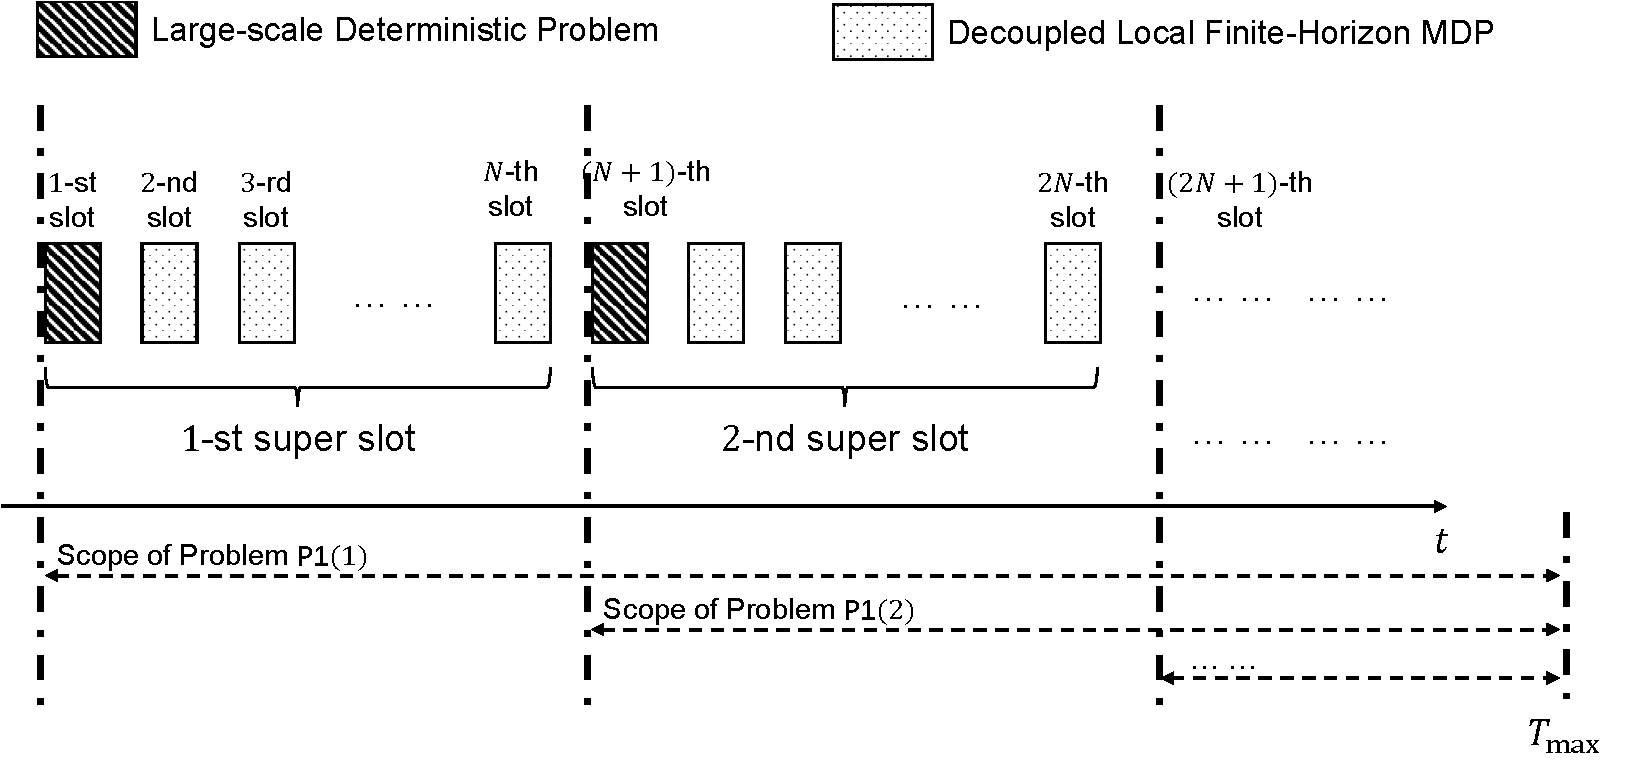
\includegraphics[width=0.90\textwidth]{optimizer-framework.pdf}
    \caption{The illustration of the {\fwName} optimizer framework.}
    \label{fig:optimizer_framework}
\end{figure*}

\section{{\fwName} Simulator for Transition Probability Training}
\label{sec:framework}

The waypoint transition probabilities $\Pr\bracket{\vec{d}_{m,t+1}|\vec{d}_{m,t}}$ ($\forall m\in\carSet$) in \eqref{eqn:trans_prob} depend on the routes, the road topology, the microscopic traffic behaviors and etc, which are usually difficult to measure in advance.
A mismatching of the trajectories' statistics would lead to a biased estimation of the value function defined in \eqref{eqn:p1_val}, and degrade the performance of the optimized scheduling policy. To our best knowledge, there is currently no analytical model for the vehicles' trajectory prediction.
Therefore, we develop the {\fwName} simulator to simulate the trajectories of {\IAVs} for arbitrary traffic scenario, so that the waypoint transition probabilities $\Pr\bracket{\vec{d}_{m,t+1}|\vec{d}_{m,t}}$ can be trained in an offline manner.

The {\fwName} simulator integrates two well-known autonomous driving simulators, namely SUMO \cite{SUMO} and CARLA \cite{CARLA}.
CARLA is the open-source simulator based on Unreal Engine \cite{unrealengine}, which provides customized road topologies and vehicle types following the OpenDRIVE specification \cite{OpenDRIVE}.
On the other hand, SUMO provides the traffic management of vehicles with well-defined microscopic traffic flow model.
Based on them, the procedure to train the transition probabilities is given as follows.

\textbf{Road Topology and Traffic Initialization.} In order to simulate the random traffic on the particular scenario, we use CARLA to generate the target road map and leverage the program \emph{ActivityGen} provided by SUMO to generate random traffic demands according to the road map. The traffic demands can be customized by adjusting the following statistics: population distribution, working hours, car-holding rate, vehicular statistics and etc.
The study \cite{sumo-accuracy-mdpi} shows that the traffic flow generated by SUMO could match the traffic conditions of the real world on usual weekdays.

\textbf{Trajectory Dataset Generation.} Based on the above road map and traffic demands, the trajectories of all vehicles can be generated and recorded.
Let $\mathcal{X}_{m} $ be the set of vehicles running on the route of the $m$-th {\IAV} in all the simulation trials, and $$ \vec{x}^{(i)}_{m} = \Paren{ \vec{d}^{(i)}_{m,1}, \vec{d}^{(i)}_{m,2}, \dots }$$ be the trajectory of the $ i $-th vehicle in $\mathcal{X}_{m}$, where $\vec{d}^{(i)}_{m,t} \in \tjSet_{m}$ is the position in the $ t $-th time slot.

\textbf{Waypoint Transition Matrix Training.} Based on the trajectory dataset $ \{\vec{x}^{(i)}_{m} | \forall i,m\} $, the transition matrices for all {\IAVs} waypoint $\{\TransD_{m}| \forall m\}$ defined in equation \eqref{eqn:trans_mat} can be obtained as follows. 
\begin{align*}
    \Paren{\TransD_{m}}_{j,k} = 
        \frac{
            \sum_{t,i} \indicator\bracket{ \vec{d}^{(i)}_{t+1}=\vec{w}_{m,k}, \vec{d}^{(i)}_{t}=\vec{w}_{m,j} }
        }{
            \sum_{t,i}\sum_{l} \indicator \bracket{ \vec{d}^{(i)}_{t+1}=\vec{w}_{m,l}, \vec{d}^{(i)}_{t}=\vec{w}_{m,j} }
        }, \forall j,k.
\end{align*}
As a remark note that the trajectory dataset generation and waypoint transition matrix training are conducted in an offline manner before the uplink transmission, the {\fwName} simulator would have sufficient time to ensure a large number of trajectory samples. 

\begin{figure*}[t]
    \begin{eqnarray}
            \sum_{\tau=kN+1}^{T} g_{\tau}\Paren{
                \mathbb{E}_{\Stat_{\tau}} \Bracket{ \Stat_{\tau} | \Stat_{kN+1} }, \vec{A}_{\tau}
            } 
            &\approx&
            T + \omega \sum_{\tau=kN+1}^{T} \sum_{m\in\carSet} \gamma_{m,\tau}
            2^\frac{r_{m,\tau}}{\gamma_{m,\tau}T_s B_0} 
            \times \xi_{m,\tau} \mathbb{E}_{\Stat_{\tau}} \Bracket{ l_{m,\tau}^{\epsilon}~|~\Stat_{kN+1} } \nonumber\\
            &\define&    F_k\Paren{ T, \mat{R}^{(k,T)}, \mat{\Gamma}^{(k,T)} }
            \label{eqn:fk}
    \end{eqnarray}
    \hrulefill
\end{figure*}

\section{{\fwName} Optimizer for Decentralized Scheduling}
\label{sec:new_framework}

The joint policy optimization for the {\IAVs} in problem {\bf P1} suffers from the {\it curse of dimensionality} \cite{mdp-huang,mdp-lv}.
This is because the transmission time and throughput allocation of each {\IAV} in each time slot depend on the global system state (aggregation of the states of all {\IAVs}), whose support grows exponentially with respect to the {\IAV} number. It can be observed that if the transmission time allocation of all {\IAVs} $\{\gamma_{m,t}|\forall m,t\}$ is predetermined, the throughput allocation of each {\IAV} in all the time slots can be optimized without the consideration of other {\IAVs}' states. However, fixing the the transmission time allocation of all {\IAVs} before the model uploading would degrade the performance, as they could not be adjusted according to the real-time positions and remaining information bits of all {\IAVs}.

In order to reduce the computational complexity and meanwhile maintain the performance gain of dynamic programming, a dynamic decoupling method is proposed for the {\fwName} optimizer in this section. The framework is illustrated in Fig. \ref{fig:optimizer_framework}, where every $N$ time slots is organized as a {\it super slot} and the online optimization consists of the following two time scales.
\begin{itemize}
    \item Super slot scale: the transmission time allocation of all {\IAVs} for the remaining time slots is periodically optimized at the beginning of each super slot. Such optimization will be approximated as a deterministic optimization problem based on the global system state at the beginning of each super slot.
    \item Slot scale: based on transmission time allocation, the optimization of throughput allocation policy of each {\IAV} for all the remaining time slots can be decoupled as a local finite-horizon MDP with tractable state space. The approximate expressions of local value functions will be derived, such that each {\IAV} can evaluate them and determine the throughput allocation in each slot without the effort of offline value iteration.
\end{itemize}

\subsection{Super Slot Scale Optimization}
Without loss of generality, we consider the scheduling since the $k$-th super slot (from the $(kN+1)$-th time slot), where $k=1,2,\dots$. The policy optimization of problem {\bf P1} for all the remaining time slots given the global system state $\Stat_{kN+1}$ reduces to the following sub-problem:
\begin{align}
    \textbf{P1$(k)$:}
    \nonumber\\ 
    &\min_{ \Policy_{kN+1}, \dots, \Policy_\T }
        \sum_{\tau=kN+1}^{\T}  \mathbb{E}_{\Stat_{\tau}} \Bracket{
            g_{\tau}\paren{ \Stat_{\tau}, \vec{A}_{\tau} } | \Stat_{kN+1}
        } \nonumber
    \\ \nonumber
    \text{s.t.~~} &\text{\eqref{eqn:p1_cons_second}, \eqref{eqn:p1_cons_last}, \eqref{eqn:p1_cons_first}},
    \\
    & \sum_{ \tau=\max\paren{kN+1,T_{\text{comp},m}} }^{ \T } r_{m,\tau} \geq {u}_{m,kN+1}, \forall m\in\carSet,
    \label{eqn:p1p_cons_last}
\end{align}
where the last constraint \eqref{eqn:p1p_cons_last} is to ensure all the data in the uplink queues of {\IAVs} should be delivered.


In the optimization of super slot scale, the average trajectories are used as the representatives to optimize the time slot allocation, such that the dynamic programming of problem \textbf{P1$(k)$} can be simplified to a deterministic optimization problem.
Note that
\begin{align}
    \sum_{\tau=kN+1}^{\T} g_{\tau}\Paren{
        \mathbb{E}_{\Stat_{\tau}}\Bracket{ \Stat_{\tau} | \Stat_{kN+1} }, \vec{A}_{\tau}
    }
    \label{eqn:cost_approx}
\end{align}
represents the system cost with the average trajectory
\begin{align}
    \Paren{
        \mathbb{E}\Bracket{ \vec{d}_{m,kN+1} | \vec{d}_{m,kN+1} },
        \dots,
        \mathbb{E}\Bracket{ \vec{d}_{m,T} | \vec{d}_{m,kN+1} }
    }
\end{align}
of the $m$-th {\IAV} ($\forall m\in\carSet$) since the $k$-th super slot. Approximating the objective by \eqref{eqn:cost_approx}, the policy optimization in problem \textbf{P1$(k)$} can be simplified into the following deterministic optimization of transmission time and throughput for the above average trajectories.
    \begin{align}
        \textbf{P2$(k)$:~} &
        ~~~\Paren{T^{(k,*)}, \mat{R}^{(k,*)}, \mat{\Gamma}^{(k,*)} }\nonumber \\
        & = \arg\min_{ T, \mat{R}^{(k,T)}, \mat{\Gamma}^{(k,T)} } F_k\Paren{ T, \mat{R}^{(k,T)}, \mat{\Gamma}^{(k,T)} }\nonumber
            \\
        &\text{s.t.~} \text{ \eqref{eqn:p1_cons_second}, \eqref{eqn:p1_cons_last}, \eqref{eqn:p1_cons_first},}
        \\
    & \sum_{ \tau=kN+1 }^{ T } r_{m,\tau} \geq {u}_{m,kN+1} \forall m\in\carSet, \label{eqn:constraint_T}
    \end{align}
where
$$
\mat{\Gamma}^{(k,T)} \define [ \gamma^{(k)}_{m,kN+\tau} ]_{1 \leq m \leq M, 1 \leq \tau \leq T-kN} \in \domR^{M \times (T-kN)}
$$
and
$$\mat{R}^{(k,T)} \define [ r^{(k)}_{m,kN+\tau}]_{1 \leq m \leq M, 1 \leq \tau \leq T-kN} \in \domR^{M \times (T-kN)}$$
are the aggregation matrices of time and throughput allocations of all the remaining time slots for the above average trajectories, respectively. $T$ denotes the number of slots in the scheduling period. $F_k(\cdot)$ is defined in \eqref{eqn:fk}, where the high-SNR approximation on power consumption
\begin{align}
    p_{m,t} \approx \xi_{m,t} l_{m,t}^{\epsilon} 2^{\frac{ r_{m,t} }{ \gamma_{m,t} T_{s} B_0 }},
\end{align}
with $\xi_{m,t} = \frac{N_0}{\kappa \sigma^\epsilon} 2^{-\mathbb{E}_{h_{m,t}}\bracket{\log_2{|h_{m,t}|^2}}}$ is used.


The  algorithm for the super slot scale optimization in problem \textbf{P2$(k)$} is discussed in Section \ref{sec:kernel-policy}.
Its solution is denoted as
$$\mat{\Gamma}^{(k,*)}=[\gamma^{(k,*)}_{m,\tau+kN}]_{1 \leq m \leq M, 1 \leq \tau \leq T^{(k,*)}-kN}$$
and
$$\mat{R}^{(k,*)}=[r^{(k,*)}_{m,\tau+kN}]_{1 \leq m \leq M, 1 \leq \tau \leq T^{(k,*)}-kN},$$
where $$\Brace{ \vecG{\gamma}^{(k,*)}_{m,\tau} | \forall m\in\carSet, \tau=kN+1,\dots,(k+1)N }$$ are adopted as the time allocation of the $k$-th super slot.


\noindent{\bf Remark:} {\it In high SNR region, with the optimized time $\mat{\Gamma}^{(k,*)}$ and throughput $\mat{R}^{(k,*)}$ allocations, the system cost with the average trajectory equals the average system cost with random trajectories. Thus,
\begin{align*}
F_k &\Paren{ T^{(k,*)}, \mat{R}^{(k,*)}, \mat{\Gamma}^{(k,*)}} =
\nonumber\\
&\sum_{\tau=kN+1}^{T^{(k,*)}} \mathbb{E}_{\Stat_{\tau}} \Bracket{
            g_{\tau}\paren{ \Stat_{\tau}, \gamma^{(k,*)}_{m,\tau}, r^{(k,*)}_{m,\tau}} | \Stat_{kN+1}
        }.
\end{align*}
This will be exploited to derive a non-trivial performance bound of the proposed algorithm.}

\subsection{Decoupled Optimization in Slot Scale}
In the slot scale, with the optimized time allocation $\mat{\Gamma}^{(k,*)}$ and optimized length of scheduling period $T^{(k,*)}$ in the previous part, the throughput allocation policies of {\IAVs} can be decoupled. We first define the following local throughput allocation policies for the $m$-th {\IAV} ($\forall m\in\carSet$):
\begin{align}
    \Policy^{R}_{m,t}( \Stat_{m,t} ) = r_{m,t},~t=kN+1,\dots,T^{(k,*)}.
\end{align}
Moreover, the local cost function of the $m$-th {\IAV} in the $t$-th time slot can be decoupled from (\ref{eqn:func_g})  as
\begin{align}
    g_{m,t}\Paren{ \Stat_{m,t}, \Policy^{R}_{m,t}(\Stat_{m,t}) } = \gamma^{(k,*)}_{m,t} p_{m,t}.
\end{align}
Then the optimization of the local throughput allocation policies for the $m$-th {\IAV} can be written as follows:
\begin{align}
    \textbf{P3$(k,m)$:~}
    &\min_{ \set{\Policy^{R}_{m,\tau} | \tau=kN+1,\dots,T^{(k,*)} } }
        \nonumber\\
        &\sum_{\tau=kN+1}^{T^{(k,*)}}
        \mathbb{E}_{\Stat_{m,\tau}} \Bracket{
            g_{m,\tau}\Paren{ \Stat_{m,\tau}, \Policy^{R}_{m,\tau}( \Stat_{m,\tau} ) }\nonumber
        }
    \\\nonumber
    &\text{s.t.~} \text{ \eqref{eqn:p1_cons_second}, \eqref{eqn:p1_cons_last}, \eqref{eqn:p1_cons_first}, } \nonumber\\
    & ~~~ \sum_{ \tau=\max\paren{kN+1,T_{\text{comp},m}} }^{ T^{(k,*)}} r_{m,\tau} \geq {u}_{m,kN+1}.
\end{align}

Note that the above problem \textbf{P3$(k,m)$} is a finite-horizon MDP based on the local system state, it can be optimized locally at the $m$-th {\IAV}. The analytical expressions to approximate its local value functions will be proposed. Hence, at the beginning of each slot in the $k$-th super slot, the $m$-th {\IAV} first evaluates the next slot's local value function, and then determines the throughput allocation action of the current slot  according to the current local system state. The solution will be discussed in Section \ref{sec:local-policy}.

    % \input{src/04a1-algorithm}  % algorithm with reference trajectory
    \section{Global Super-Slot-Scale Optimization}
\label{sec:kernel-policy}
The problem P2$(k)$ could be of a large scale when the number of remaining time slots is large. In this section, a large-scale optimization method is proposed.
Note that the time and throughput allocation ($\mat{\Gamma}^{(k,T)}, \mat{R}^{(k,T)}$) and scheduling period length $T$ are continuous and discrete, respectively, they can be optimized respectively. First, the optimization of P2$(k)$ given scheduling period length $T$ can be written as follows:
\begin{align}
    \textbf{P2$'(k,T)$:~}
    \min_{ \mat{R}^{(k,T)}, \mat{\Gamma}^{(k,T)} } &F_k\paren{ T, \mat{R}^{(k,T)}, \mat{\Gamma}^{(k,T)} }
    \\\nonumber
    \text{s.t.~} & \text{ \eqref{eqn:p1_cons_second}, \eqref{eqn:p1_cons_last}, \eqref{eqn:p1_cons_first}, \eqref{eqn:constraint_T} }.
\end{align}
Although the problem \textbf{P2$'(k,T)$} is convex, the conventional algorithms may not be applied due to huge complexity.
For example, the Newton interior method is of exponential computational complexity in the worst case \cite{monteiro1994}, which might be impractical for large $T$.
To address this issue, an acceleration gradient projection method \cite{Nesterov83} is adopted with convergence rate of $O(1/k^2)$ and computational complexity $O(k (M\T)^2)$, where $k$ denotes the number of iterations.

Let $\mat{R}^{(k,T)}_{0}, \mat{\Gamma}^{(k,T)}_{0}$ be an initial feasible solution satisfying the constraints \eqref{eqn:p1_cons_second}, \eqref{eqn:p1_cons_last}, \eqref{eqn:p1_cons_first}, and \eqref{eqn:constraint_T}.
Moreover, define
$$\mat{R}^{(k,T)}_{1}=\mat{R}^{(k,T)}_{0}, ~~\mat{\Gamma}^{(k,T)}_{1}=\mat{\Gamma}^{(k,T)}_{0}.$$
The problem \textbf{P2$'(k,T)$} can be solved by conducting the following two steps iteratively until convergence. 

\textbf{Step 1: Acceleration Point Calculation.}
In the $i$-th iteration ($i=1,2,3,\dots$), the acceleration points, denoted as $\widetilde{\mat{R}}^{(k,T)}_{i}$ and $\widetilde{\mat{\Gamma}}^{(k,T)}_{i}$, are chosen as the following linear combination of $(\mat{R}^{(k,T)}_{i}, \mat{R}^{(k,T)}_{i-1})$ and $(\mat{\Gamma}^{(k,T)}_{i}, \mat{\Gamma}^{(k,T)}_{i-1})$, respectively:
\begin{eqnarray*}
    &\widetilde{\mat{R}}^{(k,T)}_{i} &= \mat{R}^{(k,T)}_{i} + \frac{c_{i-1}-1}{c_{i}} \Paren{
        \mat{R}^{(k,T)}_{i} - \mat{R}^{(k,T)}_{i-1}
    }\nonumber
    \\
    &\widetilde{\mat{\Gamma}}^{(k,T)}_{i} &= \mat{\Gamma}^{(k,T)}_{i} + \frac{c_{i-1}-1}{c_{i}}  \Paren{
        \mat{\Gamma}^{(k,T)}_{i} - \mat{\Gamma}^{(k,T)}_{i-1} 
    },\nonumber
\end{eqnarray*}
where
\begin{align*}
    c_{0} = 1, c_{i} = \frac{1}{2} \Paren{ 1+\sqrt{ 1+4(c_{i-1})^2 } }.
\end{align*}

\textbf{Step 2: Update and Projection.}
Given the acceleration points, we define
$$\widebar{\mat{R}}^{(k,T)}_{i} = \widetilde{\mat{R}}^{(k,T)}_{i} - \eta \frac{\partial{F_k}}{\partial \mat{R}^{(k,T)}} \bigg|_{\widetilde{\mat{R}}^{(k,T)}_{i}}$$
and
$$\widebar{\mat{\Gamma}}^{(k,T)}_{i} = \widetilde{\mat{\Gamma}}^{(k,T)}_{i} - \eta \frac{\partial{F_k}}{\partial \mat{\Gamma}^{(k,T)}} \bigg|_{\widetilde{\mat{\Gamma}}^{(k,T)}_{i}}$$
where
\begin{align*}
    \frac{\partial{F_k}}{\partial \mat{R}^{(k,T)}} = \Bracket{
        &\xi_{m,\tau+kN} \mathbb{E}\bracket{ l_{m,\tau+kN}^{\epsilon} } \cdot
        2^{ \frac{r_{m,\tau+kN}}{\gamma_{m,\tau+kN} T_s B_0} }
        \nonumber\\
        &~~~~~~~~~~~~~~~~\cdot \paren{ \frac{\ln{2}}{T_s B_0} }
    }_{1 \leq m \leq M, 1 \leq \tau \leq T-kN},
    \\
    \frac{\partial{F_k}}{\partial \mat{\Gamma}^{(k,T)}} = \Bracket{
        &\xi_{m,\tau+kN} \mathbb{E}\bracket{ l_{m,\tau+kN}^{\epsilon} }
        \cdot 2^{ \frac{r_{m,\tau+kN}}{\gamma_{m,\tau+kN} T_s B_0} }
        \nonumber\\
        &\cdot \paren{1 - \frac{\ln{2}}{T_s B_0} \frac{r_{m,\tau+kN}}{\gamma_{m,\tau+kN}}}
    }_{1 \leq m \leq M, 1 \leq \tau \leq T-kN},
\end{align*}
 and $\eta$ is the constant gradient step size. Then the time and throughput allocations of the $i$-th iteration are updated as
\begin{align}
    \Paren{
        \mat{R}^{(k,T)}_{i+1}, &\mat{\Gamma}^{(k,T)}_{i+1}
    } = \mathcal{P}_{\C}\Paren{ \widebar{\mat{R}}^{(k,T)}_{i}, \widebar{\mat{\Gamma}}^{(k,T)}_{i} },
    \label{eqn:update_projection}
\end{align}
where $\mathcal{P}_{\C}$ denotes the projection of the matrix
$\widebar{\mat{R}}^{(k,T)}_{i}$ and $\widebar{\mat{\Gamma}}^{(k,T)}_{i}$
onto the constraint space $\C$ confined by equations \eqref{eqn:p1_cons_second}, \eqref{eqn:p1_cons_last}, \eqref{eqn:p1_cons_first} and \eqref{eqn:constraint_T}.

Specifically, let $\widebar{\gamma}^{(k,i)}_{m,\tau}$ and $\widebar{r}^{(k,i)}_{m,\tau}$ be the $(m,\tau)$-th entries of the matrices $\widebar{\mat{\Gamma}}^{(k,T)}_{i}$ and $\widebar{\mat{R}}^{(k,T)}_{i}$, respectively, the projection in \eqref{eqn:update_projection} is equivalently to the following minimization problem:
\begin{align}
    &\Paren{ \mat{R}^{(k,T)}_{i+1}, \mat{\Gamma}^{(k,T)}_{i+1} }
    = \arg\min_{ \paren{ \mat{R},\mat{\Gamma} } \in \C }
            \nonumber\\
            &~~~~~~~
            \sum_{m\in\carSet} \sum_{\tau=kN+1}^{T}
            \paren{ \widebar{\gamma}^{(k,i)}_{m,\tau} - \gamma_{m,\tau} }^{2} +
            \paren{ \widebar{r}^{(k,i)}_{m,\tau} - r_{m,\tau} }^{2}.
    \label{eqn:simplex_projection}
\end{align}
According to the proposition 2 of \cite{fast-projection}, the solution to the above projection is summarized in the following lemma.
\begin{lemma}[Alternative Projection Onto Simplex and Hyperplane]
    Let $\set{ \bar{\gamma}^{(m)}_{\tau} | \forall m\in\carSet }$ denote the descent sorting of $\set{ \bar{\gamma}^{(k,i)}_{m,\tau} | \forall m\in\carSet }$ in the $\tau$-th time slot ($\tau=kN+1,\dots,T$)
    ,
    and
    $\set{ \bar{r}^{(\tau)}_{m} | \tau=1,2,\dots,T-kN }$ denote the descent sorting of $\set{\bar{r}^{(k,i)}_{m,\tau} | \tau=kN+1,\dots,T}$ for the $m$-th {\IAV}.
    Thus,
    $\bar{\gamma}^{(1)}_{\tau} \geq \dots \geq \bar{\gamma}^{(M)}_{\tau}$ and $\bar{r}^{(1)}_{m} \geq \dots \geq \bar{r}^{(T-kN)}_{m}$.
    The solution of equation \eqref{eqn:simplex_projection} is given by
    \begin{align*}
        \mat{\Gamma}^{(k,T)}_{i+1} &= [\gamma^{(k,i+1)}_{m,kN+\tau}]_{1 \leq m \leq M, 1 \leq \tau \leq T-kN},
        \\
        \mat{R}^{(k,T)}_{i+1} &= [r^{(k,i+1)}_{m,kN+\tau}]_{1 \leq m \leq M, 1 \leq \tau \leq T-kN}.
    \end{align*}
    Moreover,
    \begin{align}
        \gamma^{(k,i+1)}_{m,\tau} = \Bracket{ \widebar{\gamma}^{(k,i)}_{m,\tau} &- \frac{\sum_{j=1}^{m'}\bar{\gamma}^{(j)}_{\tau} - 1}{m'} }^{+}
        \\
        r^{(k,i+1)}_{m,\tau} = \min\Paren{
            &\Bracket{ \widebar{r}^{(k,i)}_{m,\tau} - \frac{\sum_{j=1}^{\tau'}u_{m,t} - \bar{r}^{(j)}_{m}}{\tau'} }^{+},
            \nonumber\\
            &T_s B_0 \log_2\paren{ \frac{P_{\max}}{ \xi_{m,\tau} \mathbb{E}[l^{\epsilon}_{m,\tau}]}} \gamma^{(k,i+1)}_{m,\tau}
        }
    \end{align}
    where
    $$m' = \max_{m} \set{m: {\sum_{j=1}^{m} \bar{\gamma}^{(j)}_{\tau} - 1 } <{m} \bar{\gamma}^{(m)}_{\tau}},$$ 
    $$\tau' = \max_{\tau} \set{\tau: {\sum_{j=1}^{\tau} u_{m,t} - \bar{r}^{(j)}_{m}} <{\tau} \bar{r}^{(\tau)}_{m}}.$$
    % repeat the above projection procedures unless $\widebar{\mat{\Gamma}}^{(k)}$ and $\widebar{\mat{R}}^{(k)}$ are feasible.
\end{lemma}

Denote ${\mat{\Gamma}^{(k,T,*)}}$ and ${\mat{R}^{(k,T,*)}}$ as the optimized time and throughput allocations of problem \textbf{P2$'(k,T)$} after convergence, the optimization of scheduling period duration can be written as follows.
\begin{align}
    \textbf{P2$''(k)$:~} & \min_{T} F_{k}  \Paren{T, {\mat{\Gamma}^{(k,T,*)}}, {\mat{R}^{(k,T,*)}} }.
    \label{eqn:p2pp_k}
\end{align}
Note that the variable $T$ is an integer between $1$ and $\T$, a  bisection search algorithm is elaborated below to solve problem \textbf{P2$''(k)$}. Finally, the optimized scheduling period duration $T$ in problem \textbf{P2$''(k)$} is denoted as $T^{(k,*)}$, the corresponding optimized time and throughput allocations are denoted as $\mat{\Gamma}^{(k,*)}$ and  ${\mat{R}^{(k,*)}}$ respectively. 
\begin{algorithm}[ht]
    \caption{Bisection Search Algorithm for problem \textbf{P2$''(k)$}}\label{alg_bnb}
    \DontPrintSemicolon
    \KwOut{ $T^{(k,*)}$ }
    % \KwOut{$\{ { \gamma^{*}_{m,\tau} }, { r^{*}_{m,\tau} } | \forall m\in\carSet, \tau=kN+1,\dots,{T}^{*} \}$}
    $\tau_{l} \gets kN+1$, $\tau_{r} \gets \T$\;
     $w_{r} \gets \min F_{k}( \tau_{r}, \mat{R}_{r}, \mat{\Gamma}_{r} )$ by solving \textbf{P2$'( k,\tau_{r} )$}\;
    \While{ $\tau_{r} - \tau_{l} > 1$ }
    {
        $\tau_{mid} \gets \lfloor{ (\tau_{l} + \tau_{r})/2 }\rfloor$\;
        $w_{mid} \gets \min F_{k}( \tau_{mid}, \mat{R}_{mid}, \mat{\Gamma}_{mid} )$ by solving \textbf{P2$'( k,\tau_{mid} )$}\;
        \If{ $w_{r} - w_{mid} < 0$ }{
            $\tau_{l} \gets \tau_{mid}$\; %g(x)/energy domains, moves right
        }
        \Else{
            $\tau_{r} \gets \tau_{mid}$\; %f(x)/time domains, moves left
            $w_{r} \gets w_{mid}$\;
        }
    }
    \Return{ $T^{(k,*)} \gets \tau_{l}$ }\;
\end{algorithm}

\section{Local Slot-Scale Optimization}
\label{sec:local-policy}

In this section, the low-complexity algorithm solving the problem \textbf{P3$(k,m)$} without the offline value iteration is elaborated. Note that the local system state of the $m$-th {\IAV} consists of $\Stat_{m,t} =  ( u_{m,t}, \vec{d}_{m,t} )$, the Bellman's equations of problem \textbf{P3$(k,m)$} are given below.
\begin{align*}
    V_{m,t} & \paren{  u_{m,t}, \vec{d}_{m,t} }= \nonumber\\
    & \min_{ r_{m,t} } \gamma^{(k,*)}_{m,t} p_{m,t} + \mathbb{E}_{ \vec{d}_{m,t+1} } V_{m,t+1}\paren{  u_{m,t}-r_{m,t}, \vec{d}_{m,t+1} },
\end{align*}
where the transmission power $p_{m,t}$ is a function of $\gamma^{(k,*)}_{m,t}$, $\vec{d}_{m,t}$ and $r_{m,t}$, and the local value function of the $m$-th {\IAV} in the $t$-th time slot is given by
\begin{align}
    V_{m,t} & (u_{m,t}, \vec{d}_{m,t}) \define 
    \nonumber\\
    &\min_{ \{\Policy^{R}_{m,t}|\forall t\} } \mathbb{E} \Bracket{ \sum_{\tau=t}^{T^{(k,*)}} g_{m,t}(u_{m,t}, \vec{d}_{m,t}, \Policy^{R}_{m,t}) }.
\end{align}
For the notation convenience, we define
\begin{align}
    \widetilde{V}_{m,t+1}&\paren{u_{m,t+1}, \vec{d}_{m,t}}
    \nonumber\\
    &\define \mathbb{E}_{ \vec{d}_{m,t+1} | \vec{d}_{m,t} } V_{m,t+1}\paren{  u_{m,t+1}, \vec{d}_{m,t+1} }.
 \label{eqn:local_valfn_alt}
\end{align}
Hence, given the local value function and local system state, the optimal throughput allocation of the $m$-th {\IAV} in the $t_i$-th time slot, where  $t_i = kN + i$ and $i=1,2,\dots,N$, can be obtained via the following optimization problem.
\begin{align}
    \min_{ r_{m,t_i} } \gamma^{(k,*)}_{m,t_i} p_{m,t_i} (r_{m,t_i})+ \widetilde{V}_{m,t_i+1}\paren{u_{m,t_i}-r_{m,t_i}, \vec{d}_{m,t_i}}.
    \label{eqn:local_valfn}
\end{align}

Although the dimension of local value function is much less than the global optimization in equation \eqref{eqn:p1_blm},
the complexity of evaluating local value functions $V_{m,t}  (u_{m,t}, \vec{d}_{m,t})$ ($\forall t, u_{m,t}, \vec{d}_{m,t}$) or equivalently $\widetilde{V}_{m,t}(\cdot)$ is still high. Therefore, we propose a novel method to approximate the local value functions with the analytical expressions based on the reference throughput allocation. 
Let
$$\paren{ r^{(k,i-1)}_{m,t_i}, r^{(k,i-1)}_{m,t_i+1}, \dots, r^{(k,i-1)}_{m,T^{(k,*)}} }$$
with 
\begin{align}
    \sum_{\tau=t_i}^{T^{(k,*)}} r^{(k,i-1)}_{m,\tau} = u_{m,t_i}
    \label{eqn:reference_constraint}
\end{align}
be the reference throughput allocation for all the remaining time slots in the optimization of the $t_i$-th time slot, and
\begin{align*}
    \slide{r}^{(k,i-1)}_{m} = \paren{ r^{(k,i-1)}_{m,t_i+1}, r^{(k,i-1)}_{m,t_i+2}, \dots, r^{(k,i-1)}_{m,T^{(k,*)}} }
\end{align*}
be the corresponding reference throughput allocation for the future time slots. The optimization in equation \eqref{eqn:local_valfn} can be equivalently written as
\begin{align}
\textbf{P3$'(k,m,t_i)$:}& \min_{ \Delta r_{m,t_i} } \gamma^{(k,*)}_{m,t_i} p_{m,t_i} (r^{(k,i-1)}_{m,t_i}+\Delta r_{m,t_i}) \nonumber\\ 
 +~&\widetilde{V}_{m,t_i+1}\paren{u_{m,t_i}-r^{(k,i-1)}_{m,t_i}-\Delta r_{m,t_i}, \vec{d}_{m,t_i}}.  \label{eqn:local_valfn_delta}
 \\
 \text{s.t.~}& p_{m,t_i}( r^{(k,i-1)}_{m,t_i} + \Delta{r}_{m,t_i} ) \leq P_{\max}
\end{align}

\subsection{Local Value Function Approximation}
\label{subsec:local_valfn_approx}

In this part, we approximate the expected local value function $\widetilde{V}_{m,t_i+1}\paren{\cdot}$ in equation \eqref{eqn:local_valfn_delta} via the reference throughput allocations $\slide{r}^{(k,i-1)}_{m}$.
Let 
\begin{align}
    \widebar{G}_{m,t_i+1} & \paren{ \slide{r}^{(k,i-1)}_{m}, \vec{d}_{m,t_i} }
    \define
    \nonumber\\
    &\sum_{\tau=t_i+1}^{T^{(k,*)}}
    \mathbb{E}_{\vec{d}_{m,\tau}}\Bracket{
        \gamma^{(k,*)}_{m,\tau} p_{m,\tau}\paren{ r_{m,\tau}^{(k,i-1)}}
        ~|~\vec{d}_{m,t_i}
    }
\end{align}
denote the expected cost of $m$-th {\IAV} since the $(t_i+1)$-th time slot with the reference throughput allocations $\slide{r}^{(k,i)}_{m} $ given the current location $\vec{d}_{m,t_i}$, and
$$
\Delta{\slide{r}^{(k,i)}_{m}} = (\Delta{r}_{m,t_i+1},\dots,\Delta{r}_{m,T^{(k,*)}})
$$
be the adjustment on the reference throughput allocation.
We approximate the expected local value function $\widetilde{V}_{m,t_i+1}\paren{\cdot}$ in equation \eqref{eqn:local_valfn_delta} as follows:
\begin{align}
    \widetilde{V}_{m,t_i+1} & ( u_{m,t_i} -r^{(k,i-1)}_{m,t_i} -\Delta{r}_{m,t_i}, \vec{d}_{m,t_i} )  \approx
    \nonumber\\
     \min_{\Delta{\slide{r}^{(k,i)}_{m}}} & ~~~\widebar{G}_{m,t_i+1}\Paren{ \slide{r}^{(k,i-1)}_{m} + \Delta{\slide{r}^{(k,i)}_{m}}, \vec{d}_{m,t_i} }
    \nonumber\\
    \text{s.t.~} & ~~~ \sum_{\tau=t_i+1}^{T^{(k,*)}} \Delta{r}_{m,\tau} = \Delta{r}_{m,t_i}
    \nonumber\\
    & ~~~ \Delta{r}_{m,t_i} \times \Delta{r}_{m,\tau} \geq 0, \forall \tau = {t_i+1},\dots, T^{(k,*)}. \nonumber
\end{align}
The above first constraint is to ensure that the total number of transmission bits is $u_{m,t_i}$, and the second constraint is to limit the search space of $\Delta{\slide{r}^{(k,i)}_{m}}$. Moreover, we have the following conclusion on its asymptotic optimal solution.

\begin{lemma}
    \label{lemma:local_rate_opt}
    Define the following indexes of time slots:
     \begin{align}
        \hat{\tau}_{m} &= \arg\max_{\tau} \mathbb{E}\Bracket{ l_{m,\tau}^{\epsilon}~|~\vec{d}_{m,t_i} }
                          \cdot 2^{\frac{r^{(k,i)}_{m,\tau}}{T_s B_0 \gamma^{(k,*)}_{m,\tau}}},
        \\
        \breve{\tau}_{m} &= \arg\min_{\tau} \mathbb{E}\Bracket{ l_{m,\tau}^{\epsilon}~|~\vec{d}_{m,t_i} }
                          \cdot 2^{\frac{r^{(k,i)}_{m,\tau}}{T_s B_0 \gamma^{(k,*)}_{m,\tau}}}.
    \end{align}   
    For sufficiently small $\Delta{r}_{m,t_i}$, the following solution is asymptotically optimal:
    \begin{itemize}
        \item If $\Delta{r}_{m,t_i} > 0$, all the entries of $\Delta{\slide{r}^{(k,i)}_{m}}$ is $0$ except that $\Delta{r}_{m,\hat{\tau}_{m}} = \Delta{r}_{m,t_i}$;
        \item If $\Delta{r}_{m,t_i} < 0$, all the entries of $\Delta{\slide{r}^{(k,i)}_{m}}$ is $0$ except that $\Delta{r}_{m,\breve{\tau}_{m}} = \Delta{r}_{m,t_i}$;
    \end{itemize}
\end{lemma}
\begin{proof}
    Please refer to the Appendix \ref{append_1}.
\end{proof}
As a result, the expected value function can be approximated as follows:
\begin{align}
    &\widetilde{V}_{m,t_i+1}\paren{ u_{m,t_i}-r^{(k,i-1)}_{m,t_i}-\Delta{r}_{m,t_i}, \vec{d}_{m,t_i} }
    \nonumber\\
    &\approx
    \begin{cases}
        \widebar{G}_{m,t_i+1}\paren{ \slide{r}^{(k,i-1)}_{m} + \vec{e}_{\hat{\tau}_{m}} \Delta{r}_{m,t_i}, \vec{d}_{m,t_i} }, & \Delta{r}_{m,t_i} > 0
        \\
        \widebar{G}_{m,t_i+1}\paren{ \slide{r}^{(k,i-1)}_{m} + \vec{e}_{\breve{\tau}_{m}} \Delta{r}_{m,t_i}, \vec{d}_{m,t_i} }, & \Delta{r}_{m,t_i} < 0
    \end{cases}. \label{eqn:local-value-app}
\end{align}
In the above expressions, $\vec{e}_{\tau}$ denotes the vector whose $\tau$-th dimension is one and other dimensions are zero.

\subsection{Online Scheduling}
\label{subsec:local_opt}
With the local value function approximation in the previous part, the local throughput allocation of the $m$-th {\IAV} in the $t_i$-th slot can be determined by solving problem \textbf{P3$'(k,m,t_i)$}. We first introduce the following conclusion.
\begin{lemma}
    \label{lemma:local_approx_solution}
    With the approximation of local value function in \eqref{eqn:local-value-app}, the optimal solution of problem \textbf{P3$'(k,m,t_i)$} is within the set $\{f_{m,t_i}(\hat{\tau}_m),f_{m,t_i}(\breve{\tau}_m) \}$, where
    \begin{align}
        f_{m,t_i}(\tau_m) \define
        \min\Paren{
            &\frac{
                T_sB_0 \gamma^{(k,*)}_{m,t_i} \gamma^{(k,*)}_{m,\tau} \paren{ \log_2{ \mathbb{E}[l^{\epsilon}_{m,\tau_m}] } - \log_2{l^{\epsilon}_{m,t_i}} } 
            }{
                \gamma^{(k,*)}_{m,t_i} + \gamma^{(k,*)}_{m,\tau_m}
            }
            \nonumber\\
            &+\frac{
                r^{(k,*)}_{m,\tau_m}\gamma^{(k,*)}_{m,t_i} - r^{(k,*)}_{m,t_i}\gamma^{(k,*)}_{m,\tau_m} 
            }{
                \gamma^{(k,*)}_{m,t_i} + \gamma^{(k,*)}_{m,\tau_m}
            },
            \Delta{r}^{\max}_{m,t_i}
        },
    \end{align}
    where $p_{m,t_i}( r^{(k,i-1)}_{m,t_i} + \Delta{r}^{\max}_{m,t_i} ) = P_{\max}$.
\end{lemma}
\begin{proof}
    Please refer to the Appendix \ref{append_2}.
\end{proof}

Hence, the optimized throughput allocation of the $m$-th {\IAV} in the $t_i$-th slot is denoted by
\begin{align}
    r^{(k,i)}_{m,t_i} = r^{(k,i-1)}_{m,t_i}+f_{m,t_i}(\tau_m^*), \label{eqn:throughput}
\end{align}
where 
\begin{align}
    \tau_m^*=& \arg \min_{ \tau_m\in \{\hat{\tau}_m,\breve{\tau}_m\} } \gamma^{(k,*)}_{m,t_i} p_{m,t_i} (r^{(k,i-1)}_{m,t_i}+f_{m,t_i}(\tau_m)) \nonumber\\
 & + \widebar{G}_{m,t_i+1}\paren{ \slide{r}^{(k,i-1)}_{m} + \vec{e}_{\tau_{m}} f_{m,t_i}(\tau_m), \vec{d}_{m,t_i} }.
    \label{eqn:opt_tau}
\end{align}

\subsection{Proposed Policy and Performance Bound}
As a result of global super-slot-scale optimization and local slot-scale optimization, the proposed policy, denoted as $\Baseline$, is summarized below.
\begin{definition}[Proposed Policy $\Baseline$]
    \label{def:baseline}
    In the $t_i$-th time slot where $t_i=kN+i$ ($\forall k,i$),
    the transmission time allocation of {\IAVs} $[ \gamma^{\Baseline}_{m,t_i}]_m$ is obtained by solving problem \textbf{P2$(k)$} every super slot, and the uplink throughput allocation $[ r^{\Baseline}_{m,t_i}]_m$ is obtained from equation \eqref{eqn:throughput} with the reference throughput allocation
    $\paren{ r^{(k,i-1)}_{m,t_i}, r^{(k,i-1)}_{m,t_i+1}, \dots, r^{(k,i-1)}_{m,T^{(k,*)}} }$.
    Hence,  $$\gamma^{\Baseline}_{m,t_i}=\gamma^{(k,*)}_{m,t_i} \mbox{ and } r^{\Baseline}_{m,t_i} = r^{(k,i)}_{m,t_i}, \ \forall m.$$
\end{definition}

Although arbitrary reference throughput allocation satisfying equation \eqref{eqn:reference_constraint} can be used in the above approximation of local value function, the following initialization and iterative update of reference throughput allocation could lead to a non-trivial bound of the proposed algorithm. 
\begin{itemize}
    \item {\bf Initialization:} When $i=1$, 
    \begin{align}
        r^{(k,1)}_{m,\tau} = r^{(k,*)}_{m,\tau}, \forall \tau = t_{1}, \dots, T^{(k,*)}\nonumber,
    \end{align}
    where $r^{(k,*)}_{m,\tau}$ is obtained from problem {\bf P2}$(k)$.
    \item {\bf Update:} When $i>1$,
    \begin{align}
    r^{(k,i)}_{m,\tau} = 
    \begin{cases}
        r^{(k,i-1)}_{m,\tau} + f_{m,t_{i}}(\tau_m^*), &\tau=t_i
        \\
        r^{(k,i-1)}_{m,\tau} - f_{m,t_{i}}(\tau_m^*), &\tau=\tau^*_{m}
        \\
        r^{(k,i-1)}_{m,\tau}, &\tau \neq t_i, \tau^*_{m}
    \end{cases}
    \label{eqn:approx_solution}
\end{align}
\end{itemize}

Let $V^{\Baseline}_{t}(\Stat_{t})$ be the value function of the proposed policy $\Baseline$ with the system state $\Stat_{t}$ in the $t$-th time slot. Thus,
\begin{align}
    V^{\Baseline}_{t}(\Stat_{t}) \define  \mathbb{E}_{\Stat_{t},\dots,\Stat_{\T}}
    \Bracket{
        \sum_{\tau=t}^{\T} g_{\tau}\paren{ \Stat_{\tau}, [ \gamma^{\Baseline}_{m,t}]_m, [r^{\Baseline}_{m,t}]_m} | \Stat_{t}
    }.
    \label{eqn:val_baseline}
\end{align}
We have the following conclusion on the performance bound.

\begin{theorem}[Analytical Performance Bound]
    \label{theorem:performance_analysis}
    In the $t_i$-th time slot where $t_i=kN+i$ ($\forall k,i$),
    % for sufficiently large $P_{\max}$,
    we have
    \begin{align}
        &V^{\Baseline}_{t_i}(\Stat_{t_i})
        \nonumber\\
        &~~~~\leq T^{(k,*)} + \omega \sum_{m,\tau=t_i}^{T^{(k,*)}} \gamma^{(k,*)}_{m,\tau} \mathbb{E}\bracket{ p_{m,\tau}( \gamma^{(k,*)}_{m,\tau}, r^{(k,i-1)}_{m,\tau} ) | \Stat_{t_i} },
        \label{eqn:performance_bound}
    \end{align}
    where the RHS represents the average cost with
    time allocation $\{\gamma^{(k,*)}_{m,\tau}\}$ obtained at the start of the $k$-th super slot, and throughput allocation $\{r^{(k,i-1)}_{m,\tau}\}$ obtained in the $(t_i-1)$-th time slot.
    % time and throughput allocation $\{\gamma^{(k,*)}_{m,\tau}\}$ and $\{r^{(k,i-1)}_{m,\tau}\}$, respectively.
\end{theorem}
\begin{proof}
    Please refer to Appendix \ref{append_3}.
\end{proof}
    % algorithm with expected trajectory
    \section{Performance Evaluation}
\label{sec:simulation}
In this section, we will evaluate the performance of the proposed {\fwName} optimizer based on the data traces generated by the high-fidelity {\fwName} simulator. The road map of the {\fwName} simulator can be customized via CARLA \cite{CARLA}, and the typical \emph{Town01} map of CARLA is adopted as the simulation scenario. Moreover, the random traffic is generated via the \emph{activitygen} utility from SUMO \cite{SUMO}, where the parameters are configured as follows:
\begin{itemize}
    \item The total population is $1000$; $30\%$ in the age range $[0, 30]$, $50\%$ in the range $[30, 60]$, and $20\%$ in the range $[60, 90]$;
    \item The car holding rate is $58\%$, and the average time to drive $1$ kilometer is $360$ seconds;
    \item The working hour begins between 8:30AM and 9:00AM, and ends between 5:30PM and 6:00PM.
\end{itemize}
The simulator generates the 24-hour traffics across the whole map, and we choose the traffics from 8:30AM to 9:00AM to simulate the uplink model transmission.

In the uplink transmission, the length of one time slot is $2$ seconds and the maximum scheduling period is $200$ time slots, i.e., $T_s=2$ and $T_{\max}=200$ respectively.
There are $5$ {\IAVs}, each with a different pre-determined traffic route.
The number of remote antennas of the BS is $3$. The routes and locations of BSs are illustrated in Fig. \ref{fig:traffic_map}. The size of the model parameters is $750$ MBytes and the uploading bandwidth $B_0$ is $10$ MHz. The maximum transmission power of {\IAVs} is $P_{\max} = 5$ Watt. The typical channel parameters in urban area are adopted, i.e., the path-loss exponent $\epsilon=2.0$ and $\sigma=10.0$. Moreover,$T_{\text{comp},m}=0$ ($\forall m\in\carSet$) in the simulation.

\begin{figure}[htp!]
    \centering
    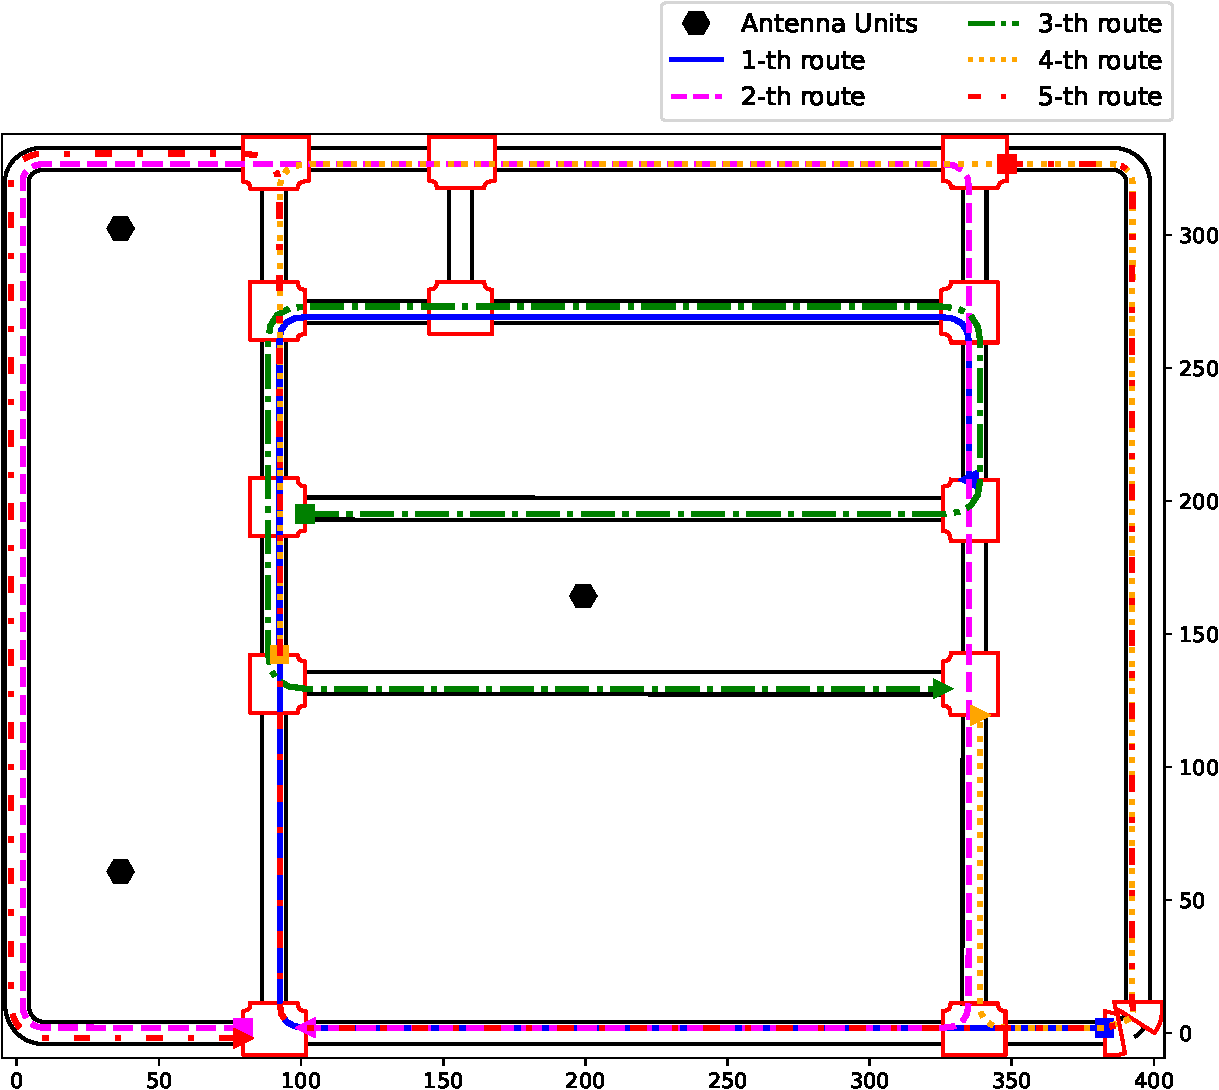
\includegraphics[width=0.45\textwidth]{fig_traffic_map.pdf}
    \caption{Illustration of the road map, {\IAV} routes, and BS locations.}
    \label{fig:traffic_map}
\end{figure}

In order to demonstrate the performance gain, we compare the proposed {\fwName} optimizer with the following benchmarks algorithms.
\begin{itemize}%<*tag:newpolicy>
    \item \revise{\textbf{Deterministic policy}: Solve the deterministic optimization problem \textbf{P2$(0)$} at the very beginning according to the average trajectories of {\IAVs}, and applied the solution in the scheduling of all the time slots.}%</tag:newpolicy>
    \item \textbf{Equal-time policy}: All the {\IAVs} are allocated with the maximum transmit power $P_{\max}$ and equal transmit time in each time slot.
    \item \textbf{Best-channel policy}: Always choose the {\IAV} with the best channel condition in each time slot, i.e., $\gamma_{m',t}=1$, $p_{m',t} = P_{\max}$, where $m' = \arg\min_{m} l_{m,t}$, $\forall t$.
    \item \textbf{Decoupled Policy}: Solve the deterministic optimization problem \textbf{P2$(0)$} at the very beginning according to the average trajectories of {\IAVs}, and apply local-slot scale optimization (problem \textbf{P3}) at each time slot based on the solution of \textbf{P2$(0)$}.
\end{itemize}

\subsection{Performance Analysis}
\label{subsec:performance}

The overall average performance of the proposed {\fwName} optimizer and the benchmarks is illustrated in Fig. \ref{fig:analyze_total_cost}, where each super slot consists of $5$ time slots.
All schemes are simulated with the same initial system state, and the average overall costs are compared. It can be observed that the average overall cost of the {\fwName} optimizer is significantly better than the equal-time policy and the best-channel policy.
\revise{
    The deterministic policy performs even worse than the equal-time policy. This is mainly because the distribution variance of {{\IAVs}}' future locations could be large at the very beginning of the scheduling. Hence, the scheduling optimization based on average trajectories may have a significant mismatch for the future time slots. Moreover, the decoupled policy performs much better than the deterministic policy.
    In the former, we use the time allocation of the deterministic policy, and apply local finite-horizon MDP to solve the power allocation for each {\IAV} respectively.
    The above performance gain demonstrates the significant benefit of dynamic programming, compared with the deterministic optimization, in the transmission with random trajectories.
}%
Finally, the performance gain of the proposed {\fwName} optimizer over the decoupled policy is due to periodic optimization of problem \textbf{P2}.


To further demonstrate the performance gap between the proposed {\fwName} optimizer and the benchmarks, we also plot the accumulated weighted cost versus time slots in Fig. \ref{fig:analyze_accumulated_cost}.


\begin{figure}
    \centering
    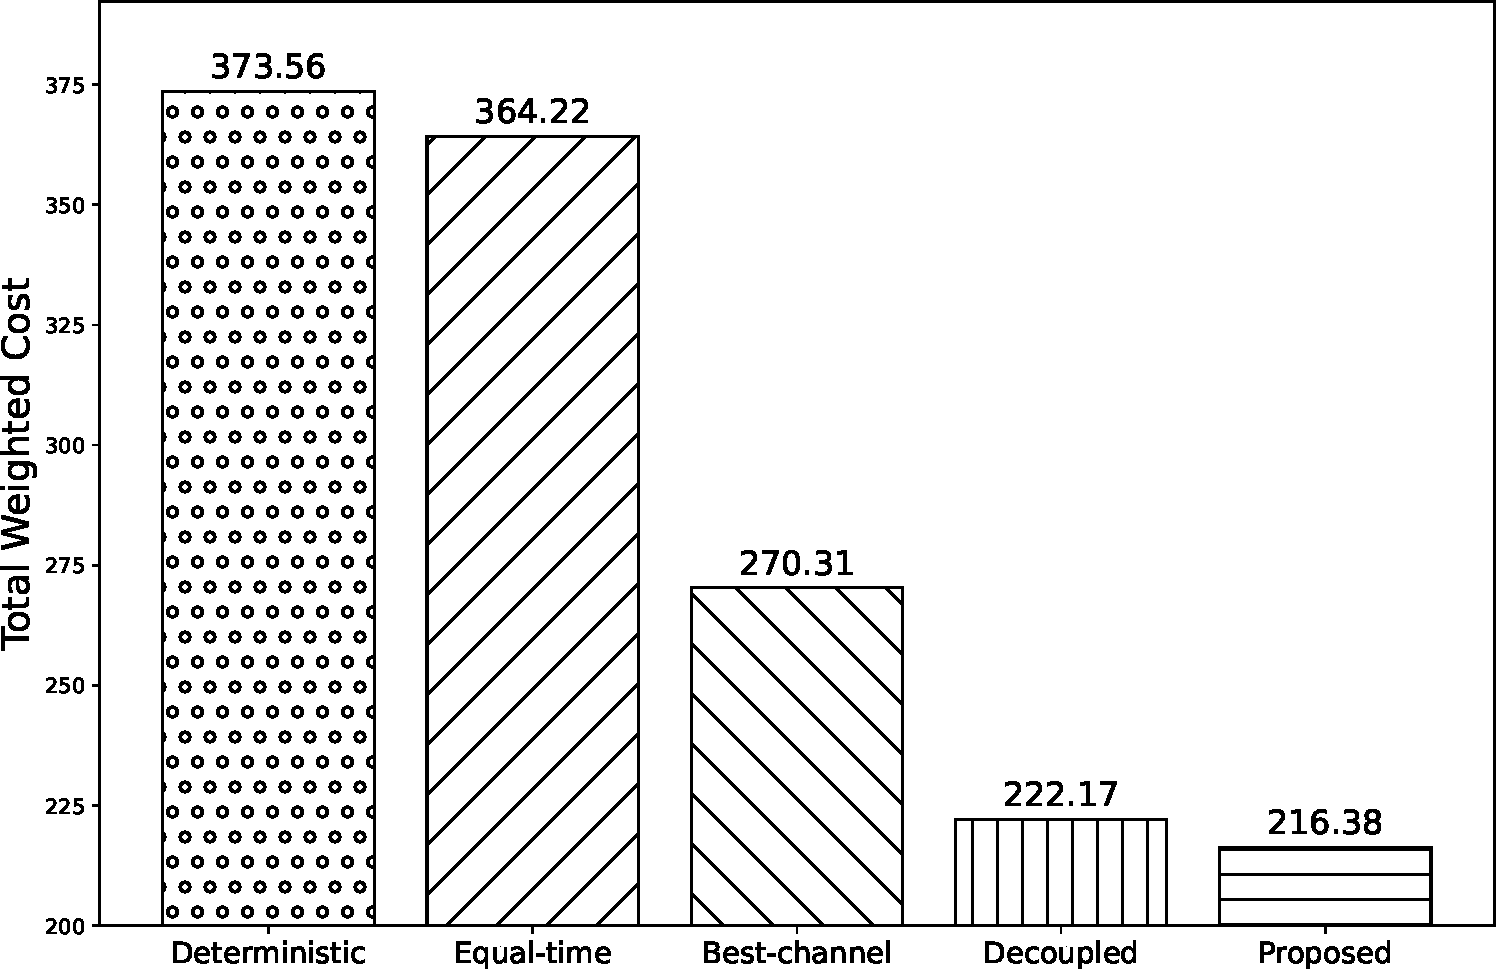
\includegraphics[width=0.45\textwidth]{analyze_cost_bar_new.pdf}
    \caption{\revise{The total weighted cost of the proposed {\fwName} optimizer and the benchmarks.}}
    \label{fig:analyze_total_cost}
\end{figure}

  
\begin{figure}
    \centering
    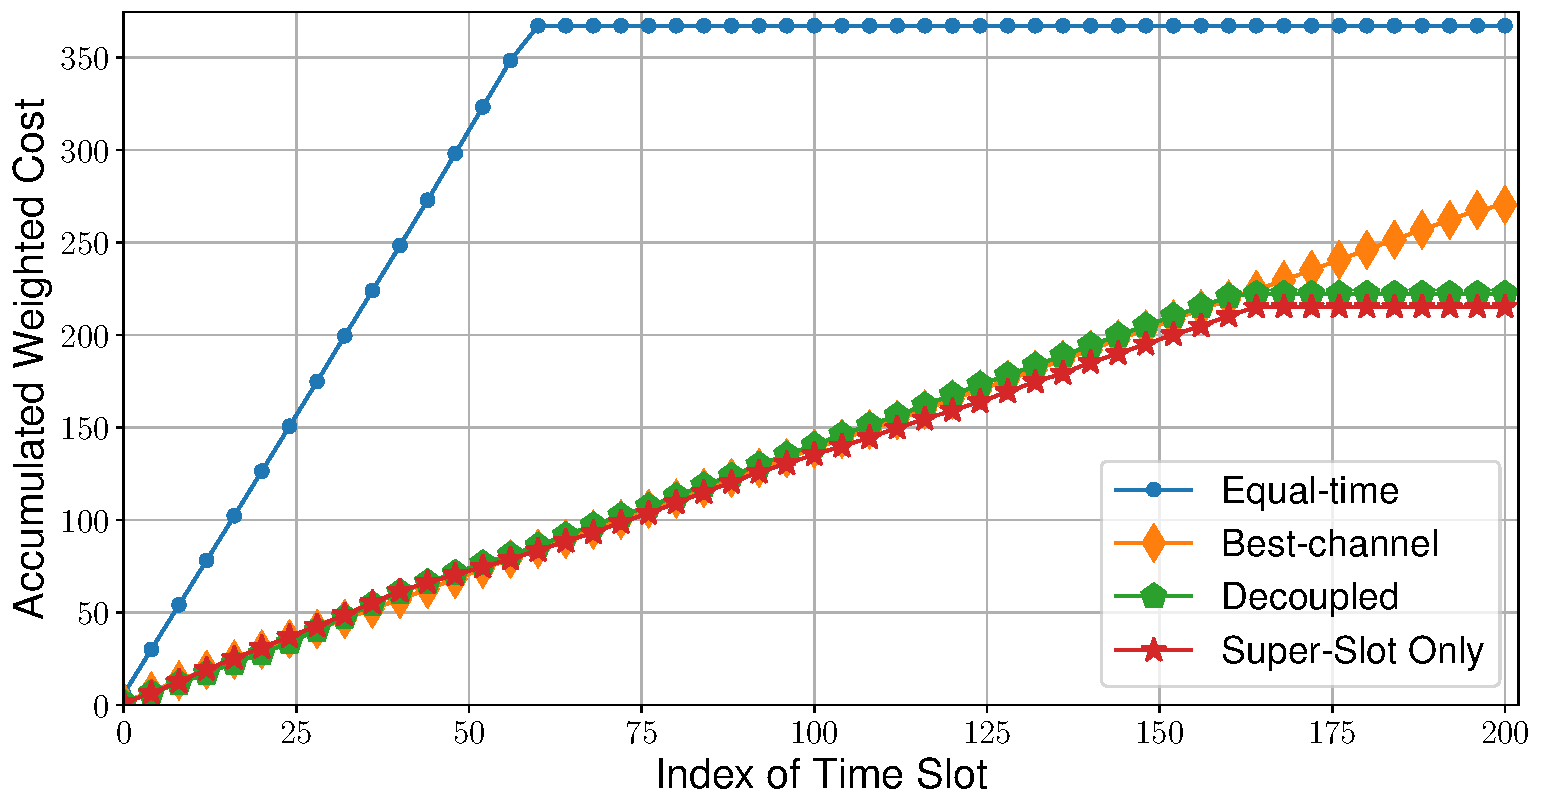
\includegraphics[width=0.45\textwidth]{analyze_accumulated_cost.pdf}
    \caption{The accumulated weighted cost versus time slots.}
    \label{fig:analyze_accumulated_cost}
\end{figure}


\subsection{Sensitivity Study}
\label{subsec:sensitivity}

In this part, the sensitivity of the performance of the proposed {\fwName} optimizer versus the system parameters is illustrated to demonstrate the robustness of the algorithm.

\noindent\textbf{Super Slot Length $N$:}
The average overall cost of the proposed {\fwName} optimizer versus different number of slots in one super slot is illustrated in Fig. \ref{fig:study_super_slot}. Smaller values of $N$ lead to more frequent super-slot scale optimization, and hence larger computational complexity. It can be observed that average overall cost decreases when decreasing $N$. Moreover, the cost suppression is trivial when $N\leq 10$.
\begin{figure}
    \centering
    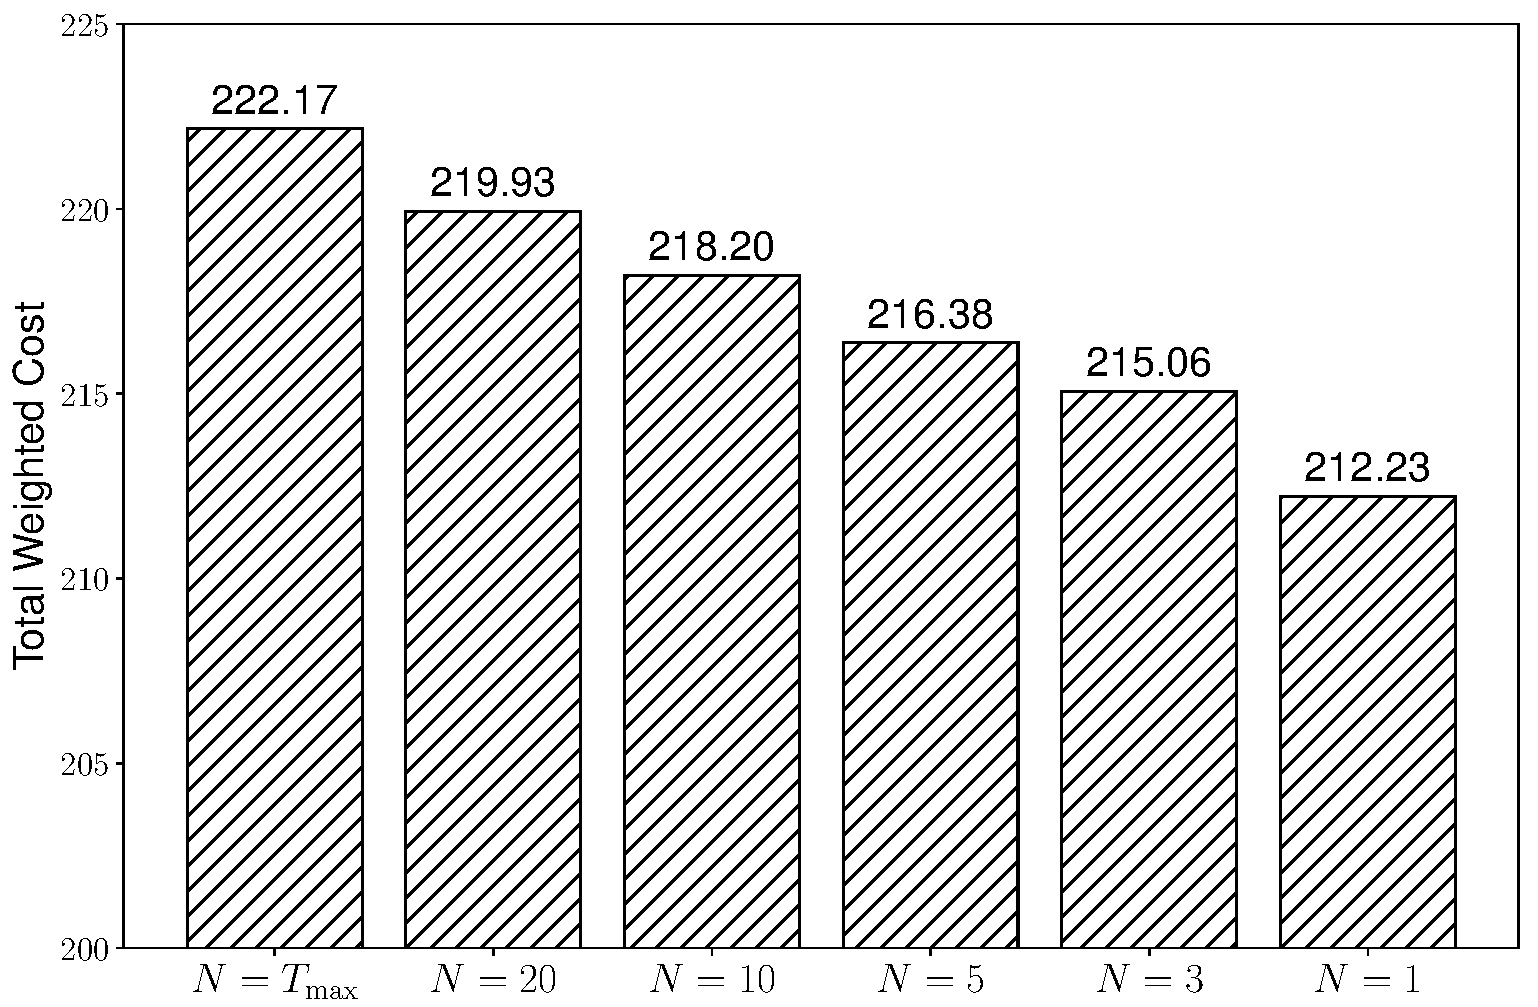
\includegraphics[width=0.45\textwidth]{study_super_slot.pdf}
    \caption{The total weighted cost w.r.t different super slot length $N$.}
    \label{fig:study_super_slot}
\end{figure}
The results show that smaller $N$ leads to better performance but higher computational complexity.

\noindent\textbf{Pareto Efficiency:}
In Fig. \ref{fig:study_pareto_efficiency}, the performance gain of the proposed {\fwName} optimizer versus different weight values $\omega$ is illustrated.
It can be observed that compared with the equal-time policy which only minimizes time consumption and the best-channel policy which only minimizes energy consumption, the proposed {\fwName} optimizer can always achieve a better trade-off between time and energy consumption.
\begin{figure}
    \centering
    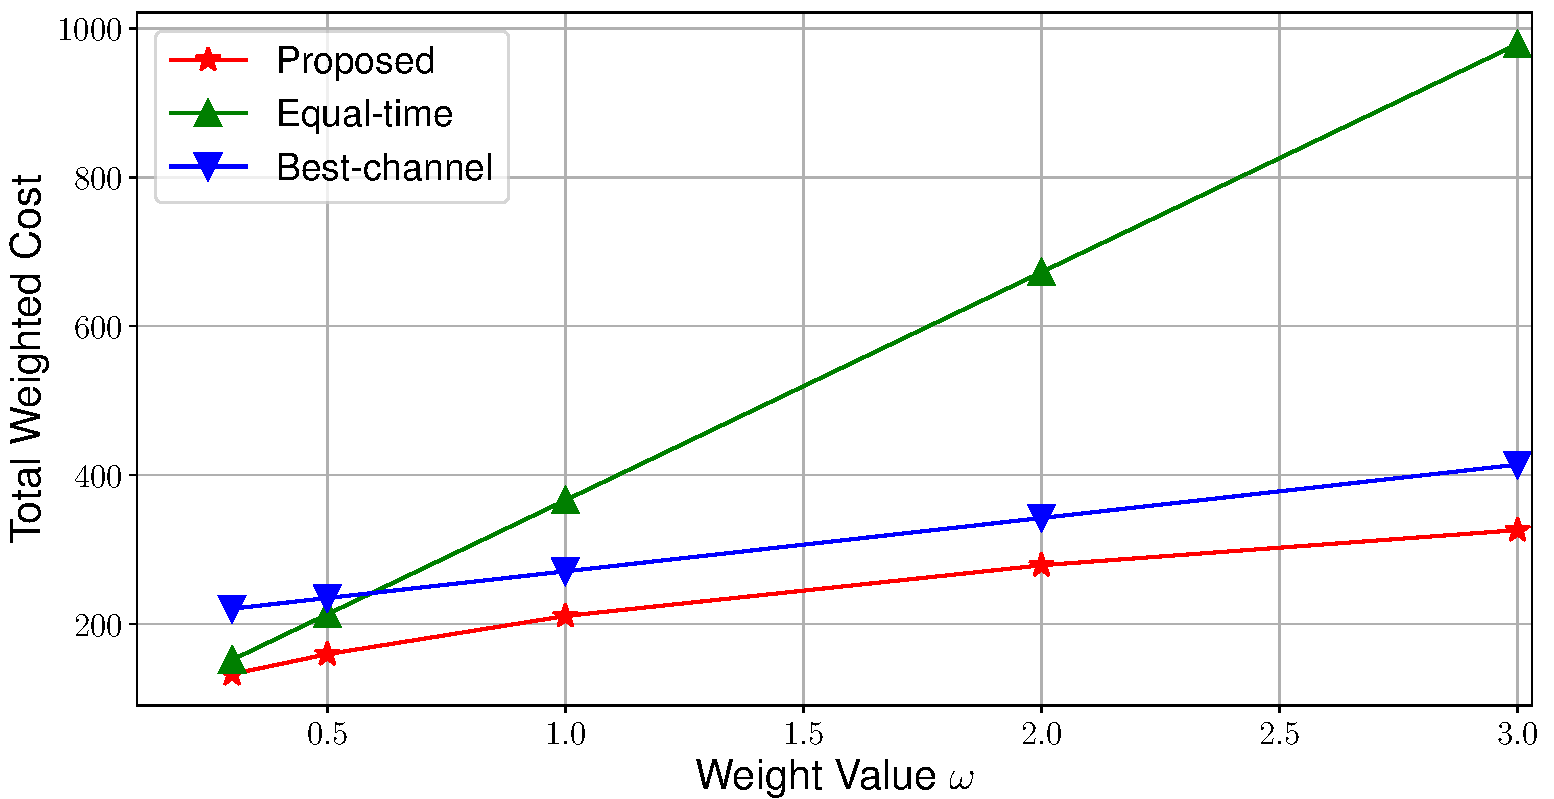
\includegraphics[width=0.45\textwidth]{study_pareto_efficiency.pdf}
    \caption{The total weighted cost of the proposed {\fwName} optimizer and the benchmarks under different weight values $\omega$.}
    \label{fig:study_pareto_efficiency}
\end{figure}

    \section{Conclusion}
\label{sec:conclusion}
In this work, a uplink scheduling framework, namely {\fwName}, is proposed to optimize the model uploading for federated learning in vehicular networks.
The proposed {\fwName} framework is composed of two components: the high-fidelity trajectory simulator and the scheduling optimizer.
With the assistance of the trajectory simulator, the stationary transition probability of the trajectories is verified, and hence, the trajectory of each {\IAV} as a time-invariant Markov chain.
The uplink transmission scheduling problem is modelled as a finite-horizon MDP.
The optimal solution suffers from the curse of dimensionality. Instead, the scheduling optimizer addresses the transmission time allocation via periodic global deterministic optimization, and the power allocation via local finite-horizon MDP. Non-trivial performance bounds are derived for the above low-complexity sub-optimal solution.
The simulation results show that the proposed solution framework can achieve both significant performance gain  compared to baselines and flexible performance-complexity trade-off.

    \appendices

\section{ Proof of Lemma \ref{lemma:local_rate_opt} }
\label{append_1}
The original optimization problem is convex, and we discuss the solution according to the sign of $\Delta{r}_{m,t_i}$. In the case of $\Delta{r}_{m,t_i} \leq 0$, we have $\Delta{r}_{m,\tau} \geq 0$ ($\tau=t_i+1, \dots, T^{(k,*)}$).
Therefore, let $\lambda \in \domR_+$ and $\vecG{\mu} \in \domR^{(T^{(k,*)}-t_i)}_+$ denote the Lagrangian multipliers, the corresponding Lagrangian of the convex optimization problem is given as follows:
\begin{align*}
    L( \Delta{\slide{r}}^{(k,i)}_{m}, \lambda, \vecG{\mu} ) =
    &\sum_{\tau=t_i+1}^{T^{(k,*)}} \gamma^{(k,*)}_{m,\tau} p_{m,\tau}( r^{(k,i)}_{m,\tau} - \Delta{r}_{m,\tau} )
    \nonumber\\
    &+ \lambda \Paren{ \sum_{\tau=t_i+1}^{T^{(k,*)}} \Delta{r}_{m,\tau} - \Delta{r}_{m,t_i} }
    \nonumber\\
    &- \sum_{j=1}^{T^{(k,*)}-t_i} \mu_{j} \Delta{r}_{m,t_i+j}.
\end{align*}

The Karush-Kuhn-Tucker (KKT) \cite{boyd-convex} conditions for the original convex optimization problem are
\begin{enumerate}
    \item \textbf{primal constraints}:
    \begin{align*}
        \sum_{\tau=t_i+1}^{T^{(k,*)}} \Delta{r}_{m,\tau} - \Delta{r}_{m,t_i} &\leq 0,
        \\
        \Delta{\slide{r}}^{(k,i)}_{m} \vecG{\mu}^T &= 0
    \end{align*}
    \item \textbf{dual constraint}:
    $$
    \lambda \geq 0
    $$
    \item \textbf{complementary slackness}:
    $$
    \lambda (\sum_{\tau=t_i+1}^{T^{(k,*)}} \Delta{r}_{m,\tau} - \Delta{r}_{m,t_i}) = 0
    $$
    \item \textbf{stationarity}:
    $$
    \nabla_{\Delta{\slide{r}}^{(k,i)}_{m}} L( \Delta{\slide{r}}^{(k,i)}_{m}, \lambda, \vec{\mu} )
    = \vec{0},
    $$
    i.e.,
    $$
    - \frac{\ln{2}}{T_sB_0} \mathbb{E}[l^{\epsilon}_{m,t_i+j}] \cdot 2^{\frac{r^{(k,i)}_{m,t_i+j} - \Delta{r}_{m,t_i+j}}{T_sB_0 \gamma^{(k,*)}_{m,t_i+j}}} + \lambda - \mu_j = 0,
    \forall j.
    $$
\end{enumerate}

According to $\Delta{\slide{r}}^{(k,i)}_{m} \vecG{\mu}^T = 0$, we have the following statement:
if $\mu_j > 0$, then $\Delta{r}_{m,t_i+j} = 0$ and
$$
\lambda < \frac{\ln{2}}{T_sB_0} \mathbb{E}[l^{\epsilon}_{m,t_i+j}] \cdot 2^{\frac{r^{(k,i)}_{m,t_i+j}}{T_sB_0 \gamma^{(k,*)}_{m,t_i+j}}}, \forall j.
$$
Moreover, we could further conclude that: $\Delta{r}_{m,t_i+j} > 0$ if
$$
\lambda \geq \frac{\ln{2}}{T_sB_0} \mathbb{E}[l^{\epsilon}_{m,t_i+j}] \cdot 2^{\frac{r^{(k,i)}_{m,t_i+j}}{T_sB_0 \gamma^{(k,*)}_{m,t_i+j}}}.
$$
% \begin{itemize}
%     \item if $\mu_j > 0$, then $\Delta{r}_{m,t_i+j} = 0$ and the following inequality holds:
%     $$
%     \lambda < \frac{\ln{2}}{T_sB_0} \mathbb{E}[l^{\epsilon}_{m,t_i+j}] \cdot 2^{\frac{r^{(k,i)}_{m,t_i+j}}{T_sB_0 \gamma^{(k,*)}_{m,t_i+j}}}, \forall j.
%     $$
%     We further conclude that: if $\lambda \geq \frac{\ln{2}}{T_sB_0} \mathbb{E}[l^{\epsilon}_{m,t_i+j}] \cdot 2^{\frac{r^{(k,i)}_{m,t_i+j}}{T_sB_0 \gamma^{(k,*)}_{m,t_i+j}}}$, then $\Delta{r}_{m,t_i+j} > 0$.
%     \item if $\mu_j = 0$, then $\Delta{r}_{m,t_i+j} \geq 0$, and we have
%     $$
%     \Delta{r}_{m,\tau} = - r^{(k,i)}_{m,\tau} + T_sB_0 \gamma^{(k,*)}_{m,\tau} \log_2{\frac{\lambda \cdot T_sB_0}{\ln{2} \mathbb{E}[l^{\epsilon}_{m,\tau}]}}, \forall \tau>t_i.
%     $$
% \end{itemize}
Therefore, $\Delta{r}_{m,t_i+j}$ ($\forall j$) is either positive or zero depending on the scalar value $\lambda$.
Hence, for sufficiently small $\Delta{r}_{m,t_i}$ w.r.t non-trivial optimal solution $\lambda^* > 0$, there is only one non-zero rate allocation whose index is given below.
$$
\hat{\tau}_{m} = \arg\max_{\tau} \mathbb{E}\Bracket{ l_{m,\tau}^{\epsilon}~|~\vec{d}_{m,t_i} }
                          \cdot 2^{\frac{r^{(k,i)}_{m,\tau}}{T_sB_0 \gamma^{(k,*)}_{m,\tau}}}.
$$

Similarly, in the case of $\Delta{r}_{m,t_i} \ge 0$, let $\Delta{\slide{r}}^{(k,i)'}_{m} = - \Delta{\slide{r}}_{m,t_i}$, we have the expression of Lagrangian $L'(\cdot)$ w.r.t $\Delta{\slide{r}}^{(k,i)'}_{m,t_i}$ as follows:
\begin{align*}
    L'( \Delta{\slide{r}}^{(k,i)'}_{m}, \lambda, \vecG{\mu} ) =
    &\sum_{\tau=t_i+1}^{T^{(k,*)}} \gamma^{(k,*)}_{m,\tau} p_{m,\tau}( r^{(k,i)}_{m,\tau} + \Delta{r}'_{m,\tau} )
    \nonumber\\
    &- \lambda \Paren{ \sum_{\tau=t_i+1}^{T^{(k,*)}} \Delta{r}_{m,\tau} - \Delta{r}_{m,t_i} }
    \nonumber\\
    &- \sum_{j=1}^{T^{(k,*)}-t_i} \mu_{j} \Delta{r}_{m,t_i+j}.
\end{align*}
Therefore, the only difference compared to the analysis in previous case exists in stationarity constraint, where
$$
\frac{\ln{2}}{T_sB_0} \mathbb{E}[l^{\epsilon}_{m,t_i+j}] \cdot 2^{\frac{r^{(k,i)}_{m,t_i+j} - \Delta{r}'_{m,t_i+j}}{T_sB_0 \gamma^{(k,*)}_{m,t_i+j}}} + \lambda - \mu_j = 0,
    \forall j.
$$
Hence, for sufficiently small $\Delta{r}_{m,t_i}$, the index of the non-zeros rate allocation is the {\it smallest one} which satisfies the corresponding constraint, i.e.,
$$
\breve{\tau}_{m} = \arg\min_{\tau} \mathbb{E}\Bracket{ l_{m,\tau}^{\epsilon}~|~\vec{d}_{m,t_i} }
                          \cdot 2^{\frac{r^{(k,i)}_{m,\tau}}{T_sB_0 \gamma^{(k,*)}_{m,\tau}}}.
$$

\section{ Proof of Lemma \ref{lemma:local_approx_solution} }
\label{append_2}
Given the selected time slot $\tau$ in Lemma \ref{lemma:local_rate_opt}, the corresponding optimal rate allocation is given as follows:
\begin{align*}
    \min_{ \Delta{r}_{m,t_i} } &\gamma^{(k,*)}_{m,t_i} p_{m,t_i}( r^{(k,i)}_{m,t_i} + \Delta{r}_{m,t_i} )
    \nonumber\\
    &+ \gamma^{(k,*)}_{m,\tau} p_{m,\tau}( r^{(k,i)}_{m,\tau} - \Delta{r}_{m,t_i} )
    % \nonumber\\
    % \text{s.t.~}& \Delta{r}_{m,t_i} < r^{(k,i)}_{m,\tau}
    % \nonumber\\
    % & -\Delta{r}_{m,t_i} < r^{(k,i)}_{m,t_i}
\end{align*}
The solution to the above optimization problem is easy to obtain by taking its derivative w.r.t $\Delta{r}_{m,t_i}$ and setting it to zero, i.e.,
$$
\frac{\ln{2}}{T_sB_0} l^{\epsilon}_{m,t_i} 2^{\frac{r^{(k,i)}_{m,t_i} + \Delta{r}_{m,t_i}}{T_sB_0 \gamma^{(k,*)}_{m,t_i}}}
+ \frac{\ln{2}}{T_sB_0} \mathbb{E}[l^{\epsilon}_{m,\tau}] 2^{\frac{r^{(k,i)}_{m,\tau} - \Delta{r}_{m,t_i}}{T_sB_0 \gamma^{(k,*)}_{m,\tau}}} = 0,
$$
and the solution is as follows:
\begin{align*}
    \Delta{r}_{m,t_i} =
    &\frac{
        T_sB_0 \gamma^{(k,*)}_{m,t_i} \gamma^{(k,*)}_{m,\tau} \paren{ \log_2{ \mathbb{E}[l^{\epsilon}_{m,\tau}] } - \log_2{l^{\epsilon}_{m,t_i}} } 
    }{
        \gamma^{(k,*)}_{m,t_i} + \gamma^{(k,*)}_{m,\tau}
    }
    \nonumber\\
    &+ \frac{
        r^{(k,*)}_{m,\tau}\gamma^{(k,*)}_{m,t_i} - r^{(k,*)}_{m,t_i}\gamma^{(k,*)}_{m,\tau} 
    }{
        \gamma^{(k,*)}_{m,t_i} + \gamma^{(k,*)}_{m,\tau}
    }.
\end{align*}

\section{ Proof of Theorem \ref{theorem:performance_analysis} }
\label{append_3}
In the following, we show that each global or local optimization of transmit time or power according to the current system state will suppress the system cost.
In the $t_i$-th time slot where $t_i=kN+i$ ($\forall k,i$),
let 
\begin{align*}
    \bar{\Policy} = \Brace{ \gamma^{(k,*)}_{m,\tau}, r^{(k,i-1)}_{m,\tau} | \forall m\in\carSet, \tau=t_i,\dots,T^{(k,*)} }
\end{align*}
denotes the policy on the right-hand-side of equation \eqref{eqn:performance_bound}, which is a state-invariant policy.
Let
\begin{align*}
    \mat{L} \define \Paren{ \vec{d}_{t_i}, \dots, \vec{d}_{\T} }
\end{align*}
denotes the trajectory of random system states of {\IAVs} from the $t_i$-th time slot to the maximum scheduling period $\T$ where $\vec{d}_{\tau} = [ \vec{d}_{m,\tau} ]_m$ ($\forall \tau$),
and $\Baseline_{L}$ denotes the fixed proposed policy along the trajectory $\mat{L}$.
Therefore, for the fixed trajectory $\mat{\bar{l}} = ( \bar{\vec{d}}_{t_i}, \dots, \bar{\vec{d}}_{\T} )$, the proposed policy $\Baseline_{\bar{l}}$ updates the resource allocation only once at the $t_i$-th slot and we have:
\begin{align*}
    V^{\Baseline_{\bar{l}}}_{t_i}( \Stat_{t_i} ) &= g_{t_i}\Paren{ \Stat_{t_i}, \Baseline_{\bar{l}}(\Stat_{t_i}) } + \mathbb{E}\bracket{ V^{ \Baseline_{\bar{l}} }( \Stat_{t_i+1} ) }
    \nonumber\\
    &\leq g_{t_i}\Paren{ \Stat_{t_i}, \bar{\Policy}(\Stat_{t_i}) } + \mathbb{E}\bracket{ V^{ \bar{\Policy} }( \Stat_{t_i+1} ) }
    \nonumber\\
    &= T^{(k,*)} + \omega \sum_{\tau=t_i, m} \gamma^{(k,*)}_{m,\tau} \mathbb{E}\bracket{ p( \gamma^{(k,*)}_{m,\tau}, r^{(k,i-1)}_{m,\tau} ) }
\end{align*}
Moreover, let
$$
\mat{L}^{(n)} = ( \bar{\vec{d}}_{t_i}, \dots, \bar{\vec{d}}_{t_i+n-1}, \vec{d}_{t_i+n}, \dots,  \vec{d}_{\T})
$$
denote a series of trajectories where the first $n$ elements are fixed and the rest are random ($n=1,\dots,\T-t_i+1$).
Specifically, $\mat{L}^{(0)} = \mat{L}$, and $\mat{L}^{(\T-t_i+1)} = \bar{l}$ is the fixed expected trajectory.
According to the policy improvement in the solution to Problem \textbf{P2$(k)$} at the start of super slot and Problem \textbf{P3$(k,m)$} for local rate allocation, the policy update between any two adjacent time slot resembles the \emph{policy improvement} step, and we have
$V^{\Baseline_{\mat{L}^{(n)}}}_{t_i}( \Stat_{t_i} ) \leq V^{\Baseline_{\mat{L}^{(n+1)}}}_{t_i}( \Stat_{t_i} )$.
Therefore, we have the following inequality holds:
\begin{align*}
    V^{\Baseline_{\mat{L}}}_{t_i}( \Stat_{t_i} ) &\leq V^{\Baseline_{\mat{L}^{(1)}}}_{t_i}( \Stat_{t_i} )
    \nonumber\\
    &\leq \dots
    \nonumber\\
    &\leq
    V^{\Baseline_{\mat{L}^{(n)}}}_{t_i}( \Stat_{t_i} ) \leq
    V^{\Baseline_{\mat{L}^{(n+1)}}}_{t_i}( \Stat_{t_i} )
    \nonumber\\
    &\leq \dots
    \nonumber\\
    &\leq V^{\Baseline_{\mat{L}^{(\T-t_i)}}}_{t_i}( \Stat_{t_i} ) \leq V^{\Baseline_{\bar{l}}}_{t_i}( \Stat_{t_i} ).
\end{align*}
As a result, the inequality in equation \eqref{eqn:performance_bound} holds, i.e.,
\begin{align*}
    V^{\Baseline}_{t_i}( \Stat_{t_i} ) &\leq V^{\Baseline_{\bar{l}}}_{t_i}( \Stat_{t_i} )
    \nonumber\\
    &\leq T^{(k,*)} + \omega \sum_{\tau=t_i, m} \gamma^{(k,*)}_{m,\tau} \mathbb{E}\bracket{ p( \gamma^{(k,*)}_{m,\tau}, r^{(k,i-1)}_{m,\tau} ) }.
\end{align*}


    \ifCLASSOPTIONcaptionsoff
        \newpage
    \fi

    \bibliographystyle{IEEEtrans}
    \bibliography{references/related.bib}

\end{document}